\documentclass[11pt, a4paper]{article}

%----------------------------------------------------------------------------------------
%	PACKAGES
%----------------------------------------------------------------------------------------
\usepackage[utf8]{inputenc} % UTF-8 encoding
\usepackage[T1]{fontenc}    % Font encoding
\usepackage{lmodern}        % Standard scalable vector font
\usepackage{circuitikz}
\usepackage{amsmath}
\allowdisplaybreaks

\usepackage{tikz}
\usetikzlibrary{arrows.meta, positioning, shapes.geometric}

\usepackage{xcolor}         % Colors
\definecolor{umblue}{RGB}{0, 51, 102}    % Deep University Blue style
\definecolor{codegray}{rgb}{0.5,0.5,0.5}
\definecolor{codegreen}{rgb}{0,0.6,0}
\definecolor{backcolour}{rgb}{0.96,0.96,0.96}
\definecolor{keywordcolor}{rgb}{0.0, 0.0, 0.5}

\usepackage{fancyhdr}       % Headers and footers
\setlength{\headheight}{22pt}
\pagestyle{fancy}
\fancyhf{}
\lhead{\color{umblue}\small\bfseries Common Emitter Amplifier Analysis} % Left header
\rhead{\small\thepage}                               % Right header
\renewcommand{\headrulewidth}{0.4pt}
\renewcommand{\headrule}{\hbox to\headwidth{\color{umblue}\leaders\hrule height \headrulewidth\hfill}}

\usepackage{titlesec}       % Custom section titles
\titleformat{\section}
  {\color{umblue}\normalfont\Large\bfseries\sffamily}
  {\thesection}{1em}{}
\titleformat{\subsection}
  {\color{umblue}\normalfont\large\bfseries\sffamily}
  {\thesubsection}{1em}{}

\usepackage{listings}       % Code listings
\lstdefinestyle{mystyle}{
    backgroundcolor=\color{backcolour},   
    commentstyle=\color{codegreen}\itshape,
    keywordstyle=\color{keywordcolor}\bfseries,
    numberstyle=\tiny\color{codegray},
    stringstyle=\color{orange},
    basicstyle=\ttfamily\footnotesize,
    breakatwhitespace=false,         
    breaklines=true,                 
    captionpos=b,                    
    keepspaces=true,                 
    numbers=left,                    
    numbersep=5pt,                  
    showspaces=false,                
    showstringspaces=false,
    showtabs=false,                  
    tabsize=4,
    frame=lines,
    rulecolor=\color{umblue}
}
\lstset{style=mystyle}

\usepackage{tcolorbox}      % Nice boxes for theorems/notes
\newtcolorbox{infobox}[1][]{
  colback=umblue!5!white,
  colframe=umblue,
  title=#1,
  fonttitle=\bfseries\sffamily
}

\usepackage{hyperref}       % Hyperlinks
\hypersetup{
    colorlinks=true,
    linkcolor=umblue,
    filecolor=magenta,      
    urlcolor=umblue,
    pdftitle={Common Emitter Amplifier Performance Trade-off Analysis},
    pdfpagemode=FullScreen,
}

\usepackage{graphicx}       % Images
\usepackage{amsmath, amssymb} % Math
\usepackage{geometry}
\usepackage{booktabs}
\usepackage{float}
\usepackage{longtable}
\geometry{top=2.5cm, bottom=2.5cm, left=2.5cm, right=2.5cm}

%----------------------------------------------------------------------------------------
%	TITLE PAGE VARIABLES
%----------------------------------------------------------------------------------------
\newcommand{\assignmentTitle}{Common Emitter Amplifier Performance \\ Trade-off Analysis}
\newcommand{\courseCode}{KIE 1007}
\newcommand{\courseName}{Electronic Circuits I}
\newcommand{\studentName}{Lim Wei Jen}
\newcommand{\studentID}{25005784/1}
\newcommand{\submissionDate}{\today}

\begin{document}

\begin{titlepage}
	\centering
	\vspace*{2cm}
	
	{\Huge\bfseries\sffamily\color{umblue} UNIVERSITY OF MALAYA \par}
	\vspace{1cm}
	{\Large\bfseries \courseCode \par}
	{\large \courseName \par}
	\vspace{3cm}
	
	{\Huge\bfseries \assignmentTitle \par}
	\vspace{3cm}
	
	\begin{tcolorbox}[colback=white,colframe=umblue,width=0.8\textwidth,arc=0mm,boxrule=1pt]
		\centering
		\large
		\begin{tabular}{rl}
			\textbf{Name:} & \studentName \\
			\textbf{Metric No:} & \studentID \\
			\textbf{Date:} & \submissionDate
		\end{tabular}
	\end{tcolorbox}
	
	\vfill
	
    \begin{center}
        \textbf{Assessment Rubric} \\
        \vspace{1em}
        \begin{figure}[H]
            \centering
            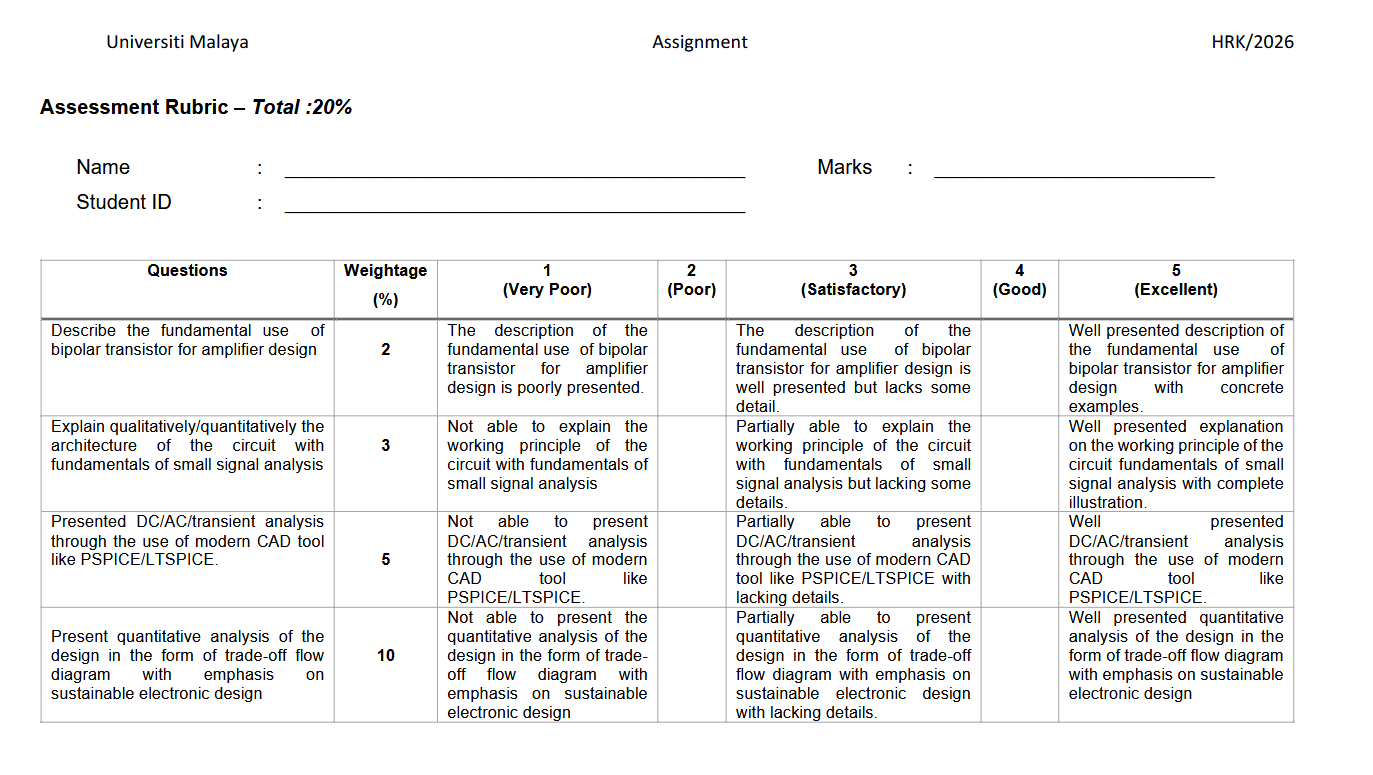
\includegraphics[width=\textwidth]{image.png}
            \label{fig:assessment_rubric}
        \end{figure}
    \end{center}

\end{titlepage}

%----------------------------------------------------------------------------------------
%	CONTENT
%----------------------------------------------------------------------------------------

\tableofcontents
\newpage

\section*{PART 1: Introduction}
\addcontentsline{toc}{section}{PART 1: Introduction}
\subsection*{1.1 The Bipolar Junction Transistor as an Amplifier}
\addcontentsline{toc}{subsection}{1.1 The Bipolar Junction Transistor as an Amplifier}

A \textbf{Bipolar Junction Transistor (BJT)} is a three-terminal semiconductor device consisting of two p-n junctions sandwiched together.
For an NPN transistor (used in this report), it has three terminals: the \textbf{Base (B)}, \textbf{Collector (C)}, and \textbf{Emitter (E)}.
The fundamental property that makes a BJT useful as an amplifier is its \emph{current-controlled current source} behaviour:

\begin{equation}
    I_C = \beta \, I_B, \qquad I_E = I_C + I_B = (1+\beta)\,I_B
\end{equation}

where $\beta$ (also written $h_{FE}$) is the \textbf{current gain} of the transistor, typically in the range 50--500 for a small-signal NPN.
This means a very small base current $I_B$ (of the order of microamperes, $\mu\text{A}$) controls a much larger collector current $I_C$ (of the order of milliamperes, mA).

\begin{infobox}[Why does a BJT amplify voltage?]
A signal source drives a small AC current into the base.
The transistor multiplies this current by $\beta$ at the collector.
This large collector current then flows through a resistor $R_C$, creating a large voltage drop $v_{out} = -i_c R_C$.
A small change in input voltage $v_{in}$ produces a much larger change in output voltage $v_{out}$ --- that is amplification.
The negative sign means the output is inverted (180° phase shift), which is the defining characteristic of the \textbf{common-emitter} configuration.
\end{infobox}

For DC biasing, the transistor must be kept in the \textbf{active region}, where $V_{BE} \approx 0.65$--$0.7\,\text{V}$ (forward-biased base-emitter junction) and $V_{CE} > V_{CE(sat)} \approx 0.2\,\text{V}$ (reverse-biased base-collector junction).
A \textbf{voltage-divider bias network} ($R_1$, $R_2$) is used in all three circuits in this report to set a stable DC base voltage, ensuring the transistor stays in the active region regardless of small variations in $\beta$.

\subsection*{1.2 Description of the Three Circuit Topologies}
\addcontentsline{toc}{subsection}{1.2 Description of the Three Circuit Topologies}

All three circuits studied in this report are \textbf{common-emitter (CE)} amplifiers built around the same NPN transistor $Q_1$.
They share a common voltage-divider bias network and coupling/bypass capacitors, but differ in how they handle the \emph{collector load} and the \emph{emitter resistor}.
The three full topologies are shown below.

Before examining each circuit, it is useful to categorise the components by type:

\begin{table}[H]
    \centering
    \caption{Classification of components in the CE amplifier circuits.}
    \renewcommand{\arraystretch}{1.3}
    \begin{tabular}{llp{7cm}}
        \toprule
        \textbf{Component Type} & \textbf{Examples} & \textbf{Role in Circuit} \\
        \midrule
        \textbf{Active} (require power to operate; control current) &
            $Q_1$ (NPN), $Q_2$, $Q_3$ (PNP) &
            Amplify or mirror current; cannot be replaced by passive elements \\
        \textbf{Passive} (store or dissipate energy) &
            $R_1$, $R_2$, $R_C$, $R_E$, $R_L$ &
            Set bias currents, provide signal load, set gain \\
        \textbf{Passive Reactive} (frequency-dependent) &
            $C_{in}$, $C_C$, $C_E$ &
            Block DC while passing AC signals; set lower cutoff frequency \\
        \bottomrule
    \end{tabular}
    \label{tab:component_types}
\end{table}

\paragraph{Circuit A --- Passive Resistive Loading (shown first below).}
This is the simplest CE amplifier.
The \textbf{collector load is a passive resistor} $R_C$.
At the emitter, a resistor $R_E$ stabilises the DC bias, while $C_E$ (the bypass capacitor) short-circuits $R_E$ at AC frequencies so that $R_E$ does \emph{not} reduce the AC gain.
All components ($R_1$, $R_2$, $R_C$, $R_E$, $C_{in}$, $C_C$, $C_E$) are passive --- the only active device is $Q_1$.
The voltage gain is $A_v \approx -\alpha (R_C \| R_L)/r_e$, which can be high, but the gain is sensitive to temperature because $r_e = V_T/I_E$ depends on temperature.

\paragraph{Circuit B --- Emitter Degeneration Loading (shown second below).}
Here the emitter resistor is split into two parts: $R_{E1}$ (upper, \emph{not} bypassed) and $R_{E2}$ (lower, bypassed by $C_E$).
At DC, both $R_{E1}$ and $R_{E2}$ contribute to biasing, setting a lower quiescent current than Circuit A.
At AC (signal frequencies), $C_E$ short-circuits $R_{E2}$ so only $R_{E1}$ remains in the signal path.
This \textbf{emitter degeneration} by $R_{E1}$ applies negative feedback: it reduces the gain to $A_v \approx -\alpha(R_C \| R_L)/(r_e + R_{E1})$, but in return it makes the gain more stable against temperature and component variation.
All components are still passive; $Q_1$ is the only active device.

\paragraph{Circuit C --- Active Loading (shown third below).}
The passive collector resistor $R_C$ is replaced by a \textbf{PNP current mirror} formed by transistors $Q_2$ and $Q_3$.
$Q_3$ is \emph{diode-connected} (its base and collector are tied together) and sets a reference current via $R_3$.
$Q_2$ mirrors this current and acts as the collector load of $Q_1$.
Because a current source has a very high output impedance ($r_{o}$), the effective AC load seen by $Q_1$'s collector is much higher than any practical resistor, driving the voltage gain towards $g_m r_o$ --- the theoretical maximum for a CE stage.
This circuit uses \textbf{both passive and active components} as the load; the current mirror transistors ($Q_2$, $Q_3$) are active semiconductors that must be powered by $V_{CC}$.


\begin{circuitikz}[american, thick]
    % Transistor
    \node[npn] (Q1) at (0,0) {};
    \node at (-0.6, 0.5) {$Q_1$}; % Label

    % Base connections and Input
    \draw (Q1.B) to[short, -*] ++(-1.5,0) coordinate(B_node);
    \draw (B_node) to[C, l=$C_{in}$, -o] ++(-2,0) node[left]{$V_{in}$};

    % Voltage divider (R1, R2) and Vcc
    \draw (B_node |- 0, 3.5) node[vcc]{$V_{cc}$} to[R, l=$R_1$, i=$I_1$] (B_node);
    \draw (B_node) to[R, l=$R_2$] (B_node |- 0, -3.5) node[ground]{};

    % Collector connections and Vcc
    \draw (Q1.C) to[short, -*] ++(0,0.5) coordinate(C_split);
    \draw (C_split |- 0, 3.5) node[vcc]{$V_{cc}$} to[R, l=$R_C$, i_=$I_2$] (C_split);

    % Output path
    \draw (C_split) to[C, l=$C_c$, -*] ++(2.5,0) coordinate(Out_node);
    \draw (Out_node) to[short, -o] ++(1.5,0) node[right]{$V_{out}$};
    
    % Load resistor
    \draw (Out_node) to[R, l_=$R_L$] (Out_node |- 0, -3.5) node[ground]{};

    % Emitter connections
    \draw (Q1.E) to[short, -*] ++(0,-0.5) coordinate(E_split);
    \draw (E_split) to[R, l=$R_E$] (E_split |- 0, -3.5) node[ground]{};
    \draw (E_split) -- ++(1.5,0) coordinate(CE_top) to[C, l=$C_E$] (CE_top |- 0, -3.5) node[ground]{};
\end{circuitikz}

\begin{circuitikz}[american, thick]
    % Transistor
    \node[npn] (Q1) at (0,0) {};
    \node at (-0.6, 0.5) {$Q_1$}; % Label

    % Base connections and Input
    \draw (Q1.B) to[short, -*] ++(-1.5,0) coordinate(B_node);
    \draw (B_node) to[C, l=$C_{in}$, -o] ++(-2,0) node[left]{$V_{in}$};

    % Voltage divider (R1, R2) and Vcc
    \draw (B_node |- 0, 3.5) node[vcc]{$V_{cc}$} to[R, l=$R_1$, i=$I_1$] (B_node);
    \draw (B_node) to[R, l=$R_2$] (B_node |- 0, -4) node[ground]{};

    % Collector connections and Vcc
    \draw (Q1.C) to[short, -*] ++(0,0.5) coordinate(C_split);
    \draw (C_split |- 0, 3.5) node[vcc]{$V_{cc}$} to[R, l=$R_C$, i_=$I_2$] (C_split);

    % Output path
    \draw (C_split) to[C, l=$C_c$, -*] ++(2.5,0) coordinate(Out_node);
    \draw (Out_node) to[short, -o] ++(1.5,0) node[right]{$V_{out}$};
    
    % Load resistor
    \draw (Out_node) to[R, l_=$R_L$] (Out_node |- 0, -4) node[ground]{};

    % Emitter connections (Degeneration: RE1, RE2, and CE)
    \draw (Q1.E) to[R, l=$R_{E1}$, -*] ++(0,-1.5) coordinate(E_mid);
    \draw (E_mid) to[R, l=$R_{E2}$] (E_mid |- 0, -4) node[ground]{};
    \draw (E_mid) -- ++(1.5,0) coordinate(CE_top) to[C, l=$C_E$] (CE_top |- 0, -4) node[ground]{};
\end{circuitikz}

\begin{circuitikz}[american, thick]
    % Main Amplifying Transistor
    \node[npn] (Q1) at (0,0) {};
    \node at (-0.6, 0.5) {$Q_1$}; 

    % Base connections and Input
    \draw (Q1.B) to[short, -*] ++(-1.5,0) coordinate(B_node);
    \draw (B_node) to[C, l=$C_{in}$, -o] ++(-2,0) node[left]{$V_{in}$};

    % Voltage divider (R1, R2) and Vcc
    \draw (B_node |- 0, 5) node[vcc]{$V_{cc}$} to[R, l=$R_1$, i=$I_1$] (B_node);
    \draw (B_node) to[R, l=$R_2$] (B_node |- 0, -4) node[ground]{};

    % Active Load (Current Mirror: Q2 and Q3)
    % Q2 is flipped horizontally (xscale=-1) so its base points right
    \node[pnp, xscale=-1] (Q2) at (0,3) {};
    \node at (-0.6, 3) {$Q_2$}; 
    \node[pnp] (Q3) at (8,3) {};
    \node at (8.6, 3) {$Q_3$};

    % Connect Q1 Collector to Q2 Collector
    \draw (Q1.C) -- (Q2.C) coordinate[midway] (C_out);
    
    % Current Mirror Connections
    \draw (Q2.B) -- (Q3.B) coordinate[pos=1] (midB);
    \draw (midB) node[circ]{} |- (Q3.C) node[circ]{}; 
    
    % Vcc connections for Active Load
    \draw (Q2.E |- 0, 5) node[vcc]{$V_{cc}$} to[short, i=$I_2$] (Q2.E);
    \draw (Q3.E |- 0, 5) node[vcc]{$V_{cc}$} to[short, i=$I_3$] (Q3.E);

    % R3 for the current mirror reference
    \draw (Q3.C) to[R, l=$R_3$] (Q3.C |- 0, -4) node[ground]{};

    % Output path
    \draw (C_out) to[C, l=$C_c$, *-*] ++(4,0) coordinate(Out_node);
    \draw (Out_node) to[short, -o] ++(1.5,0) node[right]{$V_{out}$};
    
    % Load resistor (now safely to the right of the current mirror)
    \draw (Out_node) to[R, l_=$R_L$] (Out_node |- 0, -4) node[ground]{};

    % Emitter connections (RE and CE)
    \draw (Q1.E) to[short, -*] ++(0,-0.5) coordinate(E_split);
    \draw (E_split) to[R, l=$R_E$] (E_split |- 0, -4) node[ground]{};
    \draw (E_split) -- ++(1.5,0) coordinate(CE_top) to[C, l=$C_E$] (CE_top |- 0, -4) node[ground]{};
\end{circuitikz}

\subsection*{1.3 Power Dissipation --- Where Does the Energy Go?}
\addcontentsline{toc}{subsection}{1.3 Power Dissipation}

Every component in a circuit that carries a current and has a voltage across it dissipates power as heat.
The \textbf{total power} drawn from the supply $V_{CC}$ is the most important sustainability metric, because it determines both the running cost and the heat generated.

\begin{infobox}[Derivation of $P_{total}$ = $V_{CC} I_{total}$]
The supply rail $V_{CC}$ provides current to two parallel paths: the voltage-divider branch ($I_1$ through $R_1$ and $R_2$) and the collector branch ($I_2$ through $R_C$ and the transistor).
By \textbf{Kirchhoff's Current Law (KCL)} at the $V_{CC}$ node:
\[
    I_{total} = I_1 + I_2 = \frac{V_{CC}}{R_1 + R_2} + I_C
\]
Since all this current flows from $V_{CC}$ and the negative supply terminal is ground (0\,V), the power delivered by the supply is simply:
\[
    \boxed{P_{total} = V_{CC} \times I_{total} = V_{CC}\!\left(\frac{V_{CC}}{R_1+R_2} + I_C\right)}
\]
This is a direct consequence of the definition of electrical power ($P = V \times I$) applied to the supply source.
Note that $I_C$ carries most of the power --- and $I_C$ is itself set by the biasing resistors and $\beta$, as derived in Part~2.
\end{infobox}

For Circuit C, the active-load current mirror adds a third current branch through Q2 and Q3, so:
\[
    I_{total} = I_1 + I_{C1} + I_{C3}, \quad P_{total} = V_{CC}(I_1 + 2I_C)
\]
(approximately, assuming the mirror is ideal and $I_{C2} \approx I_{C3} \approx I_{C1}$).
This explains why Circuit C draws approximately twice the collector-branch current compared to Circuit A.

\subsection*{1.4 Voltage Swing --- How Large a Signal Can We Amplify?}
\addcontentsline{toc}{subsection}{1.4 Voltage Swing}

The \textbf{voltage swing} $V_{swing}$ is the peak-to-peak output voltage range the amplifier can deliver without \emph{clipping} (distorting) the signal.
Clipping happens when the transistor is driven out of the active region --- either into \textbf{saturation} (transistor fully ON) or into \textbf{cutoff} (transistor fully OFF).

\begin{infobox}[{Derivation of $V_{swing}$ from Load-Line Analysis}]
Consider the DC load line for the collector circuit (KVL around the collector loop):
\[
    V_{CC} = I_C R_C + V_{CE} + I_E R_E
\]
The transistor can swing between two extremes:
\begin{enumerate}
    \item \textbf{Cutoff}: $I_C \to 0$, so $V_{CE} \to V_{CC}$ (maximum voltage across transistor).
    \item \textbf{Saturation}: $V_{CE} \to 0$\,V, so $I_C \to V_{CC}/(R_C + R_E)$ (maximum current).
          At saturation, the collector voltage equals $I_{C(sat)} \cdot R_E$, which from the Th\'{e}venin equivalent seen by the collector is approximately:
          \[
              V_{C(sat)} \approx V_{CC} \cdot \frac{R_2 \| R_E}{R_2 \| R_E + R_1 \| R_C}
          \]
\end{enumerate}
The transistor's quiescent (DC) operating point sits at $V_{CE}$ somewhere between these two extremes.
The output can swing by at most $v_{out}$ in either direction before hitting a limit, where:
\[
    v_{out} = \min(V_{C(sat)},\; V_{C(cutoff)}) - V_{CE}
\]
The $\min(\cdot)$ picks the \emph{closer} limit because the output cannot swing past the nearer boundary.
Since the CE amplifier is a linear (symmetric) amplifier, it can swing equally far in both the positive and negative direction, giving:
\[
    \boxed{V_{swing} = 2\,v_{out}}
\]
A well-designed amplifier places $V_{CE}$ at the midpoint between saturation and cutoff, maximising $V_{swing}$.
\end{infobox}

This is why \textbf{$V_{CE}$ is so important} from a design perspective: a transistor biased with too low a $V_{CE}$ (like Circuit A at $1.42\,\text{V}$) has very little room to swing before it saturates, while one biased near mid-supply (like Circuit C at $5.66\,\text{V}$) can swing almost the full supply range.

\subsection*{1.5 Bandwidth --- What Range of Frequencies Can Be Amplified?}
\addcontentsline{toc}{subsection}{1.5 Bandwidth}

The \textbf{bandwidth (BW)} of an amplifier is the range of frequencies over which the gain is within $1/\sqrt{2} \approx 70.7\%$ of its mid-band value (i.e., within $-3\,\text{dB}$):
\[
    \boxed{BW = f_H - f_L}
\]
where $f_H$ is the \textbf{upper} ($-3\,\text{dB}$) cutoff frequency and $f_L$ is the \textbf{lower} ($-3\,\text{dB}$) cutoff frequency.

\subsubsection*{Lower Cutoff Frequency $f_L$ --- Set by Coupling and Bypass Capacitors}

At low frequencies, the coupling capacitors ($C_{in}$, $C_C$) and the emitter bypass capacitor ($C_E$) start to behave like significant impedances.
Each capacitor, together with the resistance it sees, forms a \textbf{high-pass RC filter} with a cutoff frequency:
\[
    f_c = \frac{1}{2\pi RC}
\]
There are three such poles in the circuit:
\begin{align*}
    f_{c_{in}} &= \frac{1}{2\pi C_{in} \cdot Z_{in}} & \text{(input coupling pole)} \\
    f_{c_C}    &= \frac{1}{2\pi C_C (R_C + R_L)}      & \text{(output coupling pole)} \\
    f_{c_E}    &= \frac{1}{2\pi C_E \cdot r_e}         & \text{(emitter bypass pole)}
\end{align*}
The lower cutoff frequency is dominated by the \emph{highest} of these three poles, because whichever capacitor ``gives up'' first (stops looking like a short circuit) limits the low-frequency response:
\[
    \boxed{f_L = \max(f_{c_{in}},\; f_{c_C},\; f_{c_E})}
\]
In practice, $f_{c_E}$ is often the dominant pole because $r_e$ (a few ohms to tens of ohms) is much smaller than $R_C$ or $Z_{in}$, making $C_E$ need to be much larger to keep the pole frequency low.

\subsubsection*{Upper Cutoff Frequency $f_H$ --- Set by Internal Junction Capacitances}

At high frequencies, the transistor's own internal junction capacitances ($C_\pi$ between base and emitter, and $C_\mu$ between base and collector) begin to shunt signal current away from the output.
The most critical effect is the \textbf{Miller effect}: the base-collector capacitance $C_\mu$ is effectively \emph{multiplied} by $(1 - A_v)$ as seen from the input, because any voltage at the base is amplified to a much larger (inverted) voltage at the collector, making $C_\mu$ ``look'' much larger:
\[
    C_{Mi} = C_\mu (1 - A_v) \approx C_\mu (1 + |A_v|) \qquad \text{(Miller input capacitance)}
\]
This large effective input capacitance, combined with the Th\'{e}venin resistance driving the base ($R_{th(in)} = R_1 \| R_2 \| Z_{in}$), forms a \textbf{low-pass RC pole} that limits high-frequency gain:
\[
    f_{Hi} = \frac{1}{2\pi \, R_{th(in)} \cdot C_{in(tot)}}, \qquad C_{in(tot)} = C_\pi + C_{Mi}
\]
A similar pole exists at the output. The upper cutoff is the \emph{lower} of the two high-frequency poles (the one that limits first):
\[
    \boxed{f_H = \min(f_{Hi},\; f_{Ho})}
\]
This is why high gain and wide bandwidth are in conflict: a larger $|A_v|$ makes $C_{Mi}$ larger, which lowers $f_H$ and shrinks the bandwidth.
This fundamental limitation is captured by the \textbf{gain-bandwidth product}, which is approximately constant for a given transistor.


\section*{PART 2: DC/Transient Analysis}
\addcontentsline{toc}{section}{PART 2: DC/Transient Analysis}


\subsection*{Circuit A: Passive Resistive Loading}
\addcontentsline{toc}{subsection}{Circuit A: Passive Resistive Loading}

\begin{circuitikz}[american, thick]
    % Transistor
    \node[npn] (Q1) at (0,0) {};
    \node at (-0.6, 0.5) {$Q_1$}; % Label

    % Base connections (Voltage divider junction)
    \draw (Q1.B) to[short, -*] ++(-1.5,0) coordinate(B_node);
    
    % Voltage divider (R1, R2) and Vcc
    \draw (B_node |- 0, 3.5) node[vcc]{$V_{cc}$} to[R, l=$R_1$, i=$I_{1}$] (B_node);
    \draw (B_node) to[R, l=$R_2$] (B_node |- 0, -3.5) node[ground]{};

    % Collector connection directly to Vcc through Rc
    \draw (Q1.C) to[short] ++(0,0.5) coordinate(C_node);
    \draw (C_node |- 0, 3.5) node[vcc]{$V_{cc}$} to[R, l=$R_C$, i_=$I_{2}$] (C_node);

    % Emitter connection directly to ground through RE
    \draw (Q1.E) to[short] ++(0,-0.5) coordinate(E_node);
    \draw (E_node) to[R, l=$R_E$, i=$I_E$] (E_node |- 0, -3.5) node[ground]{};
\end{circuitikz}

\begin{align*}
    V_{TH} & = \frac{R_2}{R_1 + R_2}V_{cc}\\
    R_{TH} & = R_1 \parallel R_2 \\ \\
    \frac{R_2}{R_2+R_1}V_{CC} &= I_B (R_1 \parallel R_2) + V_{BE} + I_B(1+\beta)R_E\\
    I_B &= \frac{V_{CC}R_2/(R_1+R_2)-V_{BE}}{R_1 \parallel R_2 + (1+\beta)R_E}\\
    I_C &= \frac{V_{CC}R_2/(R_1+R_2)-V_{BE}}{R_1 \parallel R_2 + (1+\beta)R_E} \times \beta\\
    I_E &= \frac{V_{CC}R_2/(R_1+R_2)-V_{BE}}{R_1 \parallel R_2 + (1+\beta)R_E} \times (\beta + 1)\\ \\
    V_{CC} &= I_C R_C + V_{CE} + I_E R_E\\
    V_{CE} &= V_{CC} - I_C R_C - I_E R_E\\
    & = V_{CC} - \frac{V_{CC}R_2/(R_1+R_2)-V_{BE}}{R_1 \parallel R_2 + (1+\beta)R_E} \times (\beta R_C + (\beta + 1) R_E)\\ \\
    P_{total} &= V_{CC} I_{total} \textbf{ [from research]}\\
    &= V_{CC} (I_1 + I_2)\\ 
    & = V_{CC} (\frac{V_{CC}}{R_1 + R_2} + I_C)\\
    & = V_{CC} (\frac{V_{CC}}{R_1 + R_2} + \frac{V_{CC}R_2/(R_1+R_2)-V_{BE}}{R_1 \parallel R_2 + (1+\beta)R_E} \times \beta) \\ \\
    V_{C(sat)} &= V_{CC} \frac{R_2 \parallel R_E}{R_2 \parallel R_E + R_1 \parallel R_C} \\
    V_{C(cutoff)} &= V_{CC}\\
    v_{out} &= \min(V_{C(sat)}, V_{C(cutoff)}) - V_{CE} \textbf{ [from research]}\\
    V_{swing} &= 2v_{out} \textbf{ [from research]}\\
    &= 2\Big[V_{CC} \min \Big(1, \frac{R_2 \parallel R_E}{R_2 \parallel R_E + R_1 \parallel R_C}\Big) \\
    &\qquad - \Big(V_{CC} - \frac{V_{CC}R_2/(R_1+R_2)-V_{BE}}{R_1 \parallel R_2 + (1+\beta)R_E} \times (\beta R_C + (\beta + 1) R_E)\Big)\Big]
\end{align*}

\subsection*{Circuit B: Emitter Degeneration Loading}
\addcontentsline{toc}{subsection}{Circuit B: Emitter Degeneration Loading}

\begin{circuitikz}[american, thick]
    % Transistor
    \node[npn] (Q1) at (0,0) {};
    \node at (-0.6, 0.5) {$Q_1$}; % Label

    % Base connections (Voltage divider junction)
    \draw (Q1.B) to[short, -*] ++(-1.5,0) coordinate(B_node);
    
    % Voltage divider (R1, R2) and Vcc
    \draw (B_node |- 0, 3.5) node[vcc]{$V_{cc}$} to[R, l=$R_1$, i=$I_1$] (B_node);
    \draw (B_node) to[R, l=$R_2$] (B_node |- 0, -4.5) node[ground]{};

    % Collector connection directly to Vcc through Rc
    \draw (Q1.C) to[short] ++(0,0.5) coordinate(C_node);
    \draw (C_node |- 0, 3.5) node[vcc]{$V_{cc}$} to[R, l=$R_C$, i_=$I_2$] (C_node);

    % Emitter connection: RE1 and RE2 in series to ground
    \draw (Q1.E) to[R, l=$R_{E1}$, -*] ++(0,-1.5) coordinate(E_mid);
    \draw (E_mid) to[R, l=$R_{E2}$] (E_mid |- 0, -4.5) node[ground]{};
\end{circuitikz}

\begin{align*}
    V_{TH} & = \frac{R_2}{R_1 + R_2}V_{cc}\\
    R_{TH} & = R_1 \parallel R_2 \\ \\
    \frac{R_2}{R_2+R_1}V_{CC} &= I_B (R_1 \parallel R_2) + V_{BE} + I_B(1+\beta)(R_{E1}+R_{E2})\\
    I_B &= \frac{V_{CC}R_2/(R_1+R_2)-V_{BE}}{R_1 \parallel R_2 + (1+\beta)(R_{E1}+R_{E2})}\\
    I_C &= \frac{V_{CC}R_2/(R_1+R_2)-V_{BE}}{R_1 \parallel R_2 + (1+\beta)(R_{E1}+R_{E2})} \times \beta\\
    I_E &= \frac{V_{CC}R_2/(R_1+R_2)-V_{BE}}{R_1 \parallel R_2 + (1+\beta)(R_{E1}+R_{E2})} \times (\beta + 1)\\ \\
    V_{CC} &= I_C R_C + V_{CE} + I_E (R_{E1}+R_{E2})\\
    V_{CE} &= V_{CC} - I_C R_C - I_E (R_{E1}+R_{E2})\\
    & = V_{CC} - \frac{V_{CC}R_2/(R_1+R_2)-V_{BE}}{R_1 \parallel R_2 + (1+\beta)(R_{E1}+R_{E2})} \times (\beta R_C + (\beta + 1) (R_{E1}+R_{E2}))\\ \\
    P_{total} &= V_{CC} I_{total} \textbf{ [from research]}\\
    &= V_{CC} (I_1 + I_2)\\ 
    & = V_{CC} (\frac{V_{CC}}{R_1 + R_2} + I_C)\\
    & = V_{CC} (\frac{V_{CC}}{R_1 + R_2} + \frac{V_{CC}R_2/(R_1+R_2)-V_{BE}}{R_1 \parallel R_2 + (1+\beta)(R_{E1}+R_{E2})} \times \beta) \\ \\
    V_{C(sat)} &= V_{CC} \frac{R_2 \parallel (R_{E1}+R_{E2})}{R_2 \parallel (R_{E1}+R_{E2}) + R_1 \parallel R_C} \\
    V_{C(cutoff)} &= V_{CC}\\
    v_{out} &= \min(V_{C(sat)}, V_{C(cutoff)}) - V_{CE} \textbf{ [from research]}\\
    V_{swing} &= 2v_{out} \textbf{ [from research]}\\
    &= 2\Big[V_{CC} \min \Big(1, \frac{R_2 \parallel (R_{E1}+R_{E2})}{R_2 \parallel (R_{E1}+R_{E2}) + R_1 \parallel R_C}\Big) \\
    &\qquad - \Big(V_{CC} - \frac{V_{CC}R_2/(R_1+R_2)-V_{BE}}{R_1 \parallel R_2 + (1+\beta)(R_{E1}+R_{E2})} \times (\beta R_C + (\beta + 1) (R_{E1}+R_{E2}))\Big)\Big]
\end{align*}

\subsection*{Circuit C: Active Loading}
\addcontentsline{toc}{subsection}{Circuit C: Active Loading}
\begin{circuitikz}[american, thick]
    % Main Amplifying Transistor
    \node[npn] (Q1) at (0,0) {};
    \node at (-0.6, 0.5) {$Q_1$}; 

    % Base connections
    \draw (Q1.B) to[short, -*] ++(-1.5,0) coordinate(B_node);

    % Voltage divider (R1, R2) and Vcc
    \draw (B_node |- 0, 5) node[vcc]{$V_{cc}$} to[R, l=$R_1$, i=$I_1$] (B_node);
    \draw (B_node) to[R, l=$R_2$] (B_node |- 0, -4) node[ground]{};

    % Active Load (Current Mirror: Q2 and Q3)
    \node[pnp, xscale=-1] (Q2) at (0,3) {};
    \node at (-0.6, 3) {$Q_2$}; 
    \node[pnp] (Q3) at (2.5,3) {};
    \node at (3.1, 3) {$Q_3$};

    % Connect Q1 Collector to Q2 Collector
    \draw (Q1.C) -- (Q2.C);
    
    % Current Mirror Connections
    \draw (Q2.B) -- (Q3.B) coordinate[pos=0.5] (midB);
    \draw (midB) node[circ]{} |- (Q3.C) node[circ]{};
    
    % Vcc connections for Active Load
    \draw (Q2.E |- 0, 5) node[vcc]{$V_{cc}$} to[short, i=$I_E$] (Q2.E);
    \draw (Q3.E |- 0, 5) node[vcc]{$V_{cc}$} to[short, i=$I_E$] (Q3.E);

    % R3 for the current mirror reference
    \draw (Q3.C) to[R, l=$R_3$] (Q3.C |- 0, -4) node[ground]{};

    % Emitter connection (RE only)
    \draw (Q1.E) to[short] ++(0,-0.5) coordinate(E_split);
    \draw (E_split) to[R, l=$R_E$] (E_split |- 0, -4) node[ground]{};
\end{circuitikz}

\begin{align*}
    V_{TH} &= V_{CC} \frac{R_2}{R_1+R_2} \\
    R_{TH} &= R_1 \parallel R_2\\
    V_{CC} \frac{R_2}{R_1+R_2} &= I_{B1} (R_1 \parallel R_2) + V_{BE} + I_{E1} (R_E)\\
    & = I_{B1} (R_1 \parallel R_2) + V_{BE} + I_{B1}(\beta+1)R_E\\ \\
    I_{B1} &= \frac{V_{CC}\frac{R_2}{R_1+R_2}-V_{BE}}{R_1 \parallel R_2 + (\beta+1)R_E}\\
    I_{C} &= \frac{V_{CC}\frac{R_2}{R_1+R_2}-V_{BE}}{R_1 \parallel R_2 + (\beta+1)R_E} \times \beta = \beta \times I_{B1} \Rightarrow I_{B1} = I_B\\
    I_{E1} &= \frac{V_{CC}\frac{R_2}{R_1+R_2}-V_{BE}}{R_1 \parallel R_2 + (\beta+1)R_E} \times (\beta + 1)\\
    I_{E} &= I_B + I_C\\
     &= I_{B1}(\beta + 1) \Rightarrow I_{E1} = I_E \\ \\
     V_{CC} &= V_{BE} + V_{CE} + I_E R_E\\
     V_{CE} &= V_{CC} - V_{BE} - \frac{V_{CC}\frac{R_2}{R_1+R_2}-V_{BE}}{R_1 \parallel R_2 + (\beta+1)R_E} \times (\beta + 1) \times R_E\\ \\
    P_{total} &= V_{CC} I_{total} \textbf{ [from research]}\\
    &= V_{CC} (I_1 + I_2 + I_3)\\ 
    & = V_{CC} (\frac{V_{CC}}{R_1 + R_2} + 2I_E)\\
    & = V_{CC} (\frac{V_{CC}}{R_1 + R_2} + \frac{V_{CC}R_2/(R_1+R_2)-V_{BE}}{R_1 \parallel R_2 + (1+\beta)R_E} \times 2\beta)\\ \\
V_{C(sat)} &= I_E R_E\\
 &= \frac{V_{CC}\frac{R_2}{R_1+R_2}-V_{BE}}{R_1 \parallel R_2 + (\beta+1)R_E} \times (\beta + 1) \times R_E\\
 V_{C(cutoff)} &= V_{CC} - V_{BE}\\
 v_{out} &= \min(V_{C(sat)}, V_{C(cutoff)}) - V_{CE}\\
 v_{swing} &= 2v_{out}\\
 &= 2\Big(\min\Big(\frac{V_{CC}\frac{R_2}{R_1+R_2}-V_{BE}}{R_1 \parallel R_2 + (\beta+1)R_E} \times (\beta + 1) \times R_E, V_{CC} - V_{BE}\Big) \\
 &\qquad - V_{CC} - V_{BE} - \frac{V_{CC}\frac{R_2}{R_1+R_2}-V_{BE}}{R_1 \parallel R_2 + (\beta+1)R_E} \times (\beta + 1) \times R_E\Big)
\end{align*}

\subsection*{DC Analysis \& Power Dissipation Summary}
\addcontentsline{toc}{subsection}{DC Analysis \& Power Dissipation Summary}
\begin{table}[H]
    \centering
    \renewcommand{\arraystretch}{2.0}
    \begin{tabular}{@{}ll@{}}
        \toprule
        \textbf{Circuit} & \textbf{Parameters} \\
        \midrule
        \textbf{A} & 
        $\begin{aligned}
            I_B &= \frac{V_{CC}R_2/(R_1+R_2)-V_{BE}}{R_1 \parallel R_2 + (1+\beta)R_E} \\
            I_C &= \frac{V_{CC}R_2/(R_1+R_2)-V_{BE}}{R_1 \parallel R_2 + (1+\beta)R_E} \times \beta \\
            I_E &= \frac{V_{CC}R_2/(R_1+R_2)-V_{BE}}{R_1 \parallel R_2 + (1+\beta)R_E} \times (\beta + 1) \\
            P_{total} &= V_{CC} \left(\frac{V_{CC}}{R_1 + R_2} + \frac{V_{CC}R_2/(R_1+R_2)-V_{BE}}{R_1 \parallel R_2 + (1+\beta)R_E} \times \beta\right) \\
            V_{swing} &= 2\Big[V_{CC} \min \Big(1, \frac{R_2 \parallel R_E}{R_2 \parallel R_E + R_1 \parallel R_C}\Big) \\
            &\qquad - \Big(V_{CC} - \frac{V_{CC}R_2/(R_1+R_2)-V_{BE}}{R_1 \parallel R_2 + (1+\beta)R_E} \times (\beta R_C + (\beta + 1) R_E)\Big)\Big]
        \end{aligned}$ \\
        \midrule
        \textbf{B} & 
        $\begin{aligned}
            I_B &= \frac{V_{CC}R_2/(R_1+R_2)-V_{BE}}{R_1 \parallel R_2 + (1+\beta)(R_{E1}+R_{E2})} \\
            I_C &= \frac{V_{CC}R_2/(R_1+R_2)-V_{BE}}{R_1 \parallel R_2 + (1+\beta)(R_{E1}+R_{E2})} \times \beta \\
            I_E &= \frac{V_{CC}R_2/(R_1+R_2)-V_{BE}}{R_1 \parallel R_2 + (1+\beta)(R_{E1}+R_{E2})} \times (\beta + 1) \\
            P_{total} &= V_{CC} \left(\frac{V_{CC}}{R_1 + R_2} + \frac{V_{CC}R_2/(R_1+R_2)-V_{BE}}{R_1 \parallel R_2 + (1+\beta)(R_{E1}+R_{E2})} \times \beta\right) \\
            V_{swing} &= 2\Big[V_{CC} \min \Big(1, \frac{R_2 \parallel (R_{E1}+R_{E2})}{R_2 \parallel (R_{E1}+R_{E2}) + R_1 \parallel R_C}\Big) \\
            &\qquad - \Big(V_{CC} - \frac{V_{CC}R_2/(R_1+R_2)-V_{BE}}{R_1 \parallel R_2 + (1+\beta)(R_{E1}+R_{E2})} \times (\beta R_C + (\beta + 1) (R_{E1}+R_{E2}))\Big)\Big]
        \end{aligned}$ \\
        \midrule
        \textbf{C} & 
        $\begin{aligned}
            I_B &= \frac{V_{CC}\frac{R_2}{R_1+R_2}-V_{BE}}{R_1 \parallel R_2 + (\beta+1)R_E} \\
            I_C &= \frac{V_{CC}\frac{R_2}{R_1+R_2}-V_{BE}}{R_1 \parallel R_2 + (\beta+1)R_E} \times \beta \\
            I_E &= \frac{V_{CC}\frac{R_2}{R_1+R_2}-V_{BE}}{R_1 \parallel R_2 + (\beta+1)R_E} \times (\beta + 1) \\
            P_{total} &= V_{CC} \left(\frac{V_{CC}}{R_1 + R_2} + \frac{V_{CC}R_2/(R_1+R_2)-V_{BE}}{R_1 \parallel R_2 + (1+\beta)R_E} \times 2\beta\right) \\
            v_{swing} &= 2\Big(\min\Big(\frac{V_{CC}\frac{R_2}{R_1+R_2}-V_{BE}}{R_1 \parallel R_2 + (\beta+1)R_E} \times (\beta + 1) \times R_E, V_{CC} - V_{BE}\Big) \\
            &\qquad - V_{CC} - V_{BE} - \frac{V_{CC}\frac{R_2}{R_1+R_2}-V_{BE}}{R_1 \parallel R_2 + (\beta+1)R_E} \times (\beta + 1) \times R_E\Big)
        \end{aligned}$ \\
        \bottomrule
    \end{tabular}
    \caption{Summary of DC bias parameters and power dissipation across the three topologies.}
\end{table}

\section*{PART 3: AC/Transient Analysis}
\addcontentsline{toc}{section}{PART 3: AC/Transient Analysis}
\subsection*{Circuit A: Passive Resistive Loading}
\addcontentsline{toc}{subsection}{Circuit A: Passive Resistive Loading}
\begin{circuitikz}[american, thick]
    
    % Input terminal and wire
    \draw (0,0) node[ocirc]{} node[above]{$v_{in}$} to[short] (2,0);
    
    % First vertical branch (R1 || R2)
    \draw (2,0) to[R, l=$R_1||R_2$] (2,-3) node[ground]{};
    
    % Top horizontal wire with current i_b
    \draw (2,0) to[short, i=$i_b$] (4.5,0);
    
    % Second vertical branch (re)
    \draw (4.5,0) to[R, l=$r_e$, i=$i_e$] (4.5,-3) node[ground]{};
    
    % Dependent current source (drawn right-to-left so the arrow points left)
    \draw (7.5,0) to[cI, l=$\alpha i_e$] (4.5,0);
    
    % Third vertical branch (Rc || RL)
    \draw (7.5,0) to[R, l=$R_c||R_L$] (7.5,-3) node[ground]{};
    
    % Output terminal
    \draw (7.5,0) to[short, *-*] (9,0) node[above right]{$v_{out}$};
    
\end{circuitikz}

\begin{align*}
V_{out} &= -\alpha i_e (R_C \parallel R_L)\\
V_{in} &= i_e r_e\\ \\
A_v &= \frac{V_{out}}{V_{in}}\\
 &= -\frac{\alpha}{r_e}(R_C \parallel R_L)\\
 &= -\frac{\alpha (R_C \parallel R_L)(I_E)}{V_T}\\
 &= -\frac{\alpha (R_C \parallel R_L)}{V_T} \times \frac{V_{CC}R_2/(R_1+R_2)-V_{BE}}{R_1 \parallel R_2 + (1+\beta)R_E} \times (\beta + 1)\\ \\
 Z_{out} &= R_C \parallel R_L \\
 Z_{in} &= \frac{V_{in}}{i_b} \\
 &= \frac{V_{in}}{(\frac{1}{1+\beta})i_e}\\
 &= (1+\beta)r_e\\
 & = (1+\beta)\frac{V_T}{I_E}\\
 & = (1+\beta)\frac{V_T}{\frac{V_{CC}R_2/(R_1+R_2)-V_{BE}}{R_1 \parallel R_2 + (1+\beta)R_E} \times (\beta + 1)}\\
 & = \frac{V_T (R_1 \parallel R_2 + (1+\beta)R_E)}{V_{CC}R_2/(R_1+R_2)-V_{BE}}\\ \\
BW &= f_H - f_L \textbf{ [from research]}\\
f_L &= \max(f_{c_{in}}, f_{c_C}, f_{c_E}) \textbf{ [from research]}\\
X_{C_{in}} &= -\frac{1}{2\pi f_{c_{in}} C_{in}}\\ 
f_{c_{in}} &= \frac{1}{2\pi C_{in} ((1+\beta)\frac{V_T}{\frac{V_{CC}R_2/(R_1+R_2)-V_{BE}}{R_1 \parallel R_2 + (1+\beta)R_E} \times (\beta + 1)})}\\ 
f_{c_C} &= \frac{1}{2\pi C_C (R_C + R_L)}\\ 
f_{c_E} &= \frac{1}{2\pi C_E (r_e)}\\
&= \frac{I_E}{2\pi V_T C_E}\\
&= \frac{\frac{V_{CC}R_2/(R_1+R_2)-V_{BE}}{R_1 \parallel R_2 + (1+\beta)R_E} \times (\beta + 1)}{2\pi V_T C_E}\\
f_L &= \max(\frac{1}{2\pi C_{in} ((1+\beta)\frac{V_T}{\frac{V_{CC}R_2/(R_1+R_2)-V_{BE}}{R_1 \parallel R_2 + (1+\beta)R_E} \times (\beta + 1)})}, \frac{1}{2\pi C_C (R_C + R_L)}, \frac{\frac{V_{CC}R_2/(R_1+R_2)-V_{BE}}{R_1 \parallel R_2 + (1+\beta)R_E} \times (\beta + 1)}{2\pi V_T C_E})\\ \\
C_{Mi} &= C_\mu (1 - A_v)\\*
&= C_\mu \left(1 + \frac{\alpha}{r_e}(R_C \parallel R_L)\right)\\
C_{Mo} &= C_\mu \left(1 - \frac{1}{A_v}\right)\\
&= C_\mu \left(1 + \frac{r_e}{\alpha(R_C \parallel R_L)}\right)\\ \\
C_{in(tot)} &= C_\pi + C_{Mi}\\
&= C_\pi + C_\mu \left(1 + \frac{\alpha}{r_e}(R_C \parallel R_L)\right)\\
C_{out(tot)} &= C_{Mo}\\
&= C_\mu \left(1 + \frac{r_e}{\alpha(R_C \parallel R_L)}\right)\\ \\
R_{th(in)} &= R_1 \parallel R_2 \parallel Z_{in}\\
&= R_1 \parallel R_2 \parallel (1+\beta)r_e\\
R_{th(out)} &= Z_{out}\\
&= R_C \parallel R_L\\ \\
f_{Hi} &= \frac{1}{2\pi R_{th(in)} C_{in(tot)}}\\
&= \frac{1}{2\pi (R_1 \parallel R_2 \parallel (1+\beta)r_e) \left(C_\pi + C_\mu \left(1 + \frac{\alpha}{r_e}(R_C \parallel R_L)\right)\right)}\\ \\
f_{Ho} &= \frac{1}{2\pi R_{th(out)} C_{out(tot)}}\\
&= \frac{1}{2\pi (R_C \parallel R_L) C_\mu \left(1 + \frac{r_e}{\alpha(R_C \parallel R_L)}\right)}\\ \\
f_H &= \min(f_{Hi}, f_{Ho})\\
&= \min\Bigg(
    \frac{1}{2\pi (R_1 \parallel R_2 \parallel (1+\beta)(\frac{V_T}{\frac{V_{CC}R_2/(R_1+R_2)-V_{BE}}{R_1 \parallel R_2 + (1+\beta)R_E} \times (\beta + 1)}))} \\
&\qquad\qquad\qquad \times \frac{1}{\left(C_\pi + C_\mu \left(1 + \frac{\alpha}{(\frac{V_T}{\frac{V_{CC}R_2/(R_1+R_2)-V_{BE}}{R_1 \parallel R_2 + (1+\beta)R_E} \times (\beta + 1)})}(R_C \parallel R_L)\right)\right)}, \\
&\qquad \frac{1}{2\pi (R_C \parallel R_L) C_\mu \left(1 + \frac{(\frac{V_T}{\frac{V_{CC}R_2/(R_1+R_2)-V_{BE}}{R_1 \parallel R_2 + (1+\beta)R_E} \times (\beta + 1)})}{\alpha(R_C \parallel R_L)}\right)}
\Bigg) \\ \\
BW &= f_H - f_L\\
& = \min\Bigg(
    \frac{1}{2\pi (R_1 \parallel R_2 \parallel (1+\beta)(\frac{V_T}{\frac{V_{CC}R_2/(R_1+R_2)-V_{BE}}{R_1 \parallel R_2 + (1+\beta)R_E} \times (\beta + 1)}))} \\
&\qquad\qquad\qquad \times \frac{1}{\left(C_\pi + C_\mu \left(1 + \frac{\alpha}{(\frac{V_T}{\frac{V_{CC}R_2/(R_1+R_2)-V_{BE}}{R_1 \parallel R_2 + (1+\beta)R_E} \times (\beta + 1)})}(R_C \parallel R_L)\right)\right)}, \\
&\qquad \frac{1}{2\pi (R_C \parallel R_L) C_\mu \left(1 + \frac{(\frac{V_T}{\frac{V_{CC}R_2/(R_1+R_2)-V_{BE}}{R_1 \parallel R_2 + (1+\beta)R_E} \times (\beta + 1)})}{\alpha(R_C \parallel R_L)}\right)}
\Bigg) \\
&\qquad - \max\Bigg(
    \frac{1}{2\pi C_{in} ((1+\beta)\frac{V_T}{\frac{V_{CC}R_2/(R_1+R_2)-V_{BE}}{R_1 \parallel R_2 + (1+\beta)R_E} \times (\beta + 1)})}, \\
&\qquad\qquad\qquad \frac{1}{2\pi C_C (R_C + R_L)}, \\
&\qquad\qquad\qquad \frac{\frac{V_{CC}R_2/(R_1+R_2)-V_{BE}}{R_1 \parallel R_2 + (1+\beta)R_E} \times (\beta + 1)}{2\pi V_T C_E}
\Bigg)
\end{align*}

\subsection*{Circuit B: Emitter Degeneration Loading}
\addcontentsline{toc}{subsection}{Circuit B: Emitter Degeneration Loading}
\begin{circuitikz}[american, thick]
    
    % Input terminal and wire
    \draw (0,0) node[ocirc]{} node[above]{$v_{in}$} to[short] (2,0);
    
    % First vertical branch (R1 || R2)
    \draw (2,0) to[R, l=$R_1||R_2$] (2,-3) node[ground]{};
    
    % Top horizontal wire with current i_b
    \draw (2,0) to[short, i=$i_b$] (4.5,0);
    
    % Second vertical branch (re)
    \draw (4.5,0) to[R, l=$r_e + R_{E1}$, i=$i_e$] (4.5,-3) node[ground]{};
    
    % Dependent current source (drawn right-to-left so the arrow points left)
    \draw (7.5,0) to[cI, l=$\alpha i_e$] (4.5,0);
    
    % Third vertical branch (Rc || RL)
    \draw (7.5,0) to[R, l=$R_c||R_L$] (7.5,-3) node[ground]{};
    
    % Output terminal
    \draw (7.5,0) to[short, *-*] (9,0) node[above right]{$v_{out}$};
    
\end{circuitikz}

\begin{align*}
    V_{out} &= -\alpha i_e (R_C \parallel R_L)\\
    V_{in} &= i_e (r_e+R_{E1})\\ \\
    A_v &= \frac{V_{out}}{V_{in}}\\
    &= -\frac{\alpha}{(r_e+R_{E1})}(R_C \parallel R_L)\\
    &= -\frac{\alpha}{\frac{V_T}{I_E}+R_{E1}}(R_C \parallel R_L)\\
    &= -\frac{\alpha}{\frac{V_T}{\frac{V_{CC}R_2/(R_1+R_2)-V_{BE}}{R_1 \parallel R_2 + (1+\beta)(R_{E1}+R_{E2})} \times (\beta + 1)}+R_{E1}}(R_C \parallel R_L)\\ \\
 Z_{out} &= R_C \parallel R_L \\
 Z_{in} &= \frac{V_{in}}{i_b} \\
 &= \frac{V_{in}}{(\frac{1}{1+\beta})i_e}\\
 & = (1+\beta) (r_e + R_{E1})\\
 & = (1+\beta) (\frac{V_T}{I_E} + R_{E1})\\
 & = (1+\beta) (\frac{V_T}{\frac{V_{CC}R_2/(R_1+R_2)-V_{BE}}{R_1 \parallel R_2 + (1+\beta)(R_{E1}+R_{E2})} \times (\beta + 1)} + R_{E1})\\ \\
f_L &= \max(f_{c_{in}}, f_{c_C}, f_{c_E}) \textbf{ [from research]}\\
f_{c_{in}} &= \frac{1}{2\pi C_{in} ((1+\beta) (\frac{V_T}{\frac{V_{CC}R_2/(R_1+R_2)-V_{BE}}{R_1 \parallel R_2 + (1+\beta)(R_{E1}+R_{E2})} \times (\beta + 1)} + R_{E1}))}\\
f_{c_C} &= \frac{1}{2\pi C_C (R_C + R_L)}\\
f_{c_E} &= \frac{1}{2\pi C_E \left(R_{E2} \parallel \left(R_{E1} + r_e + \frac{R_1 \parallel R_2}{1+\beta}\right)\right)}\\
f_L &= \max(\frac{1}{2\pi C_{in} ((1+\beta) (\frac{V_T}{\frac{V_{CC}R_2/(R_1+R_2)-V_{BE}}{R_1 \parallel R_2 + (1+\beta)(R_{E1}+R_{E2})} \times (\beta + 1)} + R_{E1}))},\\ &\frac{1}{2\pi C_C (R_C + R_L)},\\ &\frac{1}{2\pi C_E \left(R_{E2} \parallel \left(R_{E1} + r_e + \frac{R_1 \parallel R_2}{1+\beta}\right)\right)}) \\ \\
C_{Mi} &= C_\mu (1 - A_v)\\
&= C_\mu \left(1 + \frac{\alpha(R_C \parallel R_L)}{r_e + R_{E1}}\right)\\
C_{Mo} &= C_\mu \left(1 - \frac{1}{A_v}\right)\\
&= C_\mu \left(1 + \frac{r_e + R_{E1}}{\alpha(R_C \parallel R_L)}\right)\\ \\
C_{in(tot)} &= C_\pi + C_{Mi}\\
&= C_\pi + C_\mu \left(1 + \frac{\alpha(R_C \parallel R_L)}{r_e + R_{E1}}\right)\\
C_{out(tot)} &= C_{Mo}\\
&= C_\mu \left(1 + \frac{r_e + R_{E1}}{\alpha(R_C \parallel R_L)}\right)\\ \\
R_{th(in)} &= R_1 \parallel R_2 \parallel (1+\beta)(r_e + R_{E1})\\
R_{th(out)} &= R_C \parallel R_L\\ \\
f_{Hi} &= \frac{1}{2\pi R_{th(in)} C_{in(tot)}}\\
&= \frac{1}{2\pi (R_1 \parallel R_2 \parallel (1+\beta)(\frac{V_T}{\frac{V_{CC}R_2/(R_1+R_2)-V_{BE}}{R_1 \parallel R_2 + (1+\beta)(R_{E1}+R_{E2})} \times (\beta + 1)} + R_{E1})) (C_\pi + C_\mu \left(1 + \frac{\alpha(R_C \parallel R_L)}{r_e + R_{E1}}\right))}\\
f_{Ho} &= \frac{1}{2\pi R_{th(out)} C_{out(tot)}}\\
&= \frac{1}{2\pi R_{th(out)} (C_\mu \left(1 + \frac{r_e + R_{E1}}{\alpha(R_C \parallel R_L)}\right))}\\
&= \frac{1}{2\pi R_{th(out)} (C_\mu \left(1 + \frac{(\frac{V_T}{\frac{V_{CC}R_2/(R_1+R_2)-V_{BE}}{R_1 \parallel R_2 + (1+\beta)(R_{E1}+R_{E2})} \times (\beta + 1)}) + R_{E1}}{\alpha(R_C \parallel R_L)}\right))}\\
f_H &= \min(f_{Hi}, f_{Ho})\\
&= \min\Bigg(
    \frac{1}{2\pi (R_1 \parallel R_2 \parallel (1+\beta)(\frac{V_T}{\frac{V_{CC}R_2/(R_1+R_2)-V_{BE}}{R_1 \parallel R_2 + (1+\beta)(R_{E1}+R_{E2})} \times (\beta + 1)} + R_{E1}))} \\
&\qquad\qquad\qquad \times \frac{1}{(C_\pi + C_\mu \left(1 + \frac{\alpha(R_C \parallel R_L)}{r_e + R_{E1}}\right))}, \\
&\qquad \frac{1}{2\pi R_{th(out)} (C_\mu \left(1 + \frac{(\frac{V_T}{\frac{V_{CC}R_2/(R_1+R_2)-V_{BE}}{R_1 \parallel R_2 + (1+\beta)(R_{E1}+R_{E2})} \times (\beta + 1)}) + R_{E1}}{\alpha(R_C \parallel R_L)}\right))}
\Bigg)\\
BW &= f_H - f_L\\
& = \min\Bigg(
    \frac{1}{2\pi (R_1 \parallel R_2 \parallel (1+\beta)(\frac{V_T}{\frac{V_{CC}R_2/(R_1+R_2)-V_{BE}}{R_1 \parallel R_2 + (1+\beta)(R_{E1}+R_{E2})} \times (\beta + 1)} + R_{E1}))} \\
&\qquad\qquad\qquad \times \frac{1}{(C_\pi + C_\mu \left(1 + \frac{\alpha(R_C \parallel R_L)}{r_e + R_{E1}}\right))}, \\
&\qquad \frac{1}{2\pi R_{th(out)} (C_\mu \left(1 + \frac{(\frac{V_T}{\frac{V_{CC}R_2/(R_1+R_2)-V_{BE}}{R_1 \parallel R_2 + (1+\beta)(R_{E1}+R_{E2})} \times (\beta + 1)}) + R_{E1}}{\alpha(R_C \parallel R_L)}\right))}
\Bigg) \\
&\qquad - \max\Bigg(
    \frac{1}{2\pi C_{in} ((1+\beta) (\frac{V_T}{\frac{V_{CC}R_2/(R_1+R_2)-V_{BE}}{R_1 \parallel R_2 + (1+\beta)(R_{E1}+R_{E2})} \times (\beta + 1)} + R_{E1}))}, \\
&\qquad\qquad\qquad \frac{1}{2\pi C_C (R_C + R_L)}, \\
&\qquad\qquad\qquad \frac{1}{2\pi C_E \left(R_{E2} \parallel \left(R_{E1} + r_e + \frac{R_1 \parallel R_2}{1+\beta}\right)\right)}
\Bigg)
\end{align*}

\subsection*{Circuit C: Active Loading}
\addcontentsline{toc}{subsection}{Circuit C: Active Loading}
\begin{circuitikz}[american, thick]
    % --- Input Stage ---
    \draw (-5,-2) node[circ]{} node[left]{$V_{in}$} to[short, -*] (0,-2);
    
    % R1 || R2 Biasing
    \draw (-3,-2) to[R=$R_1||R_2$] (-3,-4) node[ground]{};
    
    % --- Q1 (NPN Amplifier) ---
    % T-Model Core (NPN)
    \draw (0,0) to[cI, l=$\alpha i_{e1}$] (0,-2); 
    \draw (0,-2) to[R=$r_{e}$, i>=$i_{e1}$] (0,-4) node[ground]{}; 

    % --- Q2 (PNP Active Load) ---
    % Emitter to AC Ground
    \draw (0,4) node[ground, rotate=180]{} to[R=$r_{e}$, i>=$i_{e}$] (0,2);
    
    % T-Model Core (PNP)
    \draw (0,2) to[cI, l=$\alpha i_{e}$] (0,0); 
    
    % --- Output Stage (MOVED TO CENTER) ---
    % Main signal wire stops before the Q3 branch
    \draw (0,0) to[short, *-] (2.5,0);
    \draw (2.5,0) to[R=$R_L$] (2.5,-4) node[ground]{};
    \draw (2.5,0) to[short, *-o] (3.5,0) node[right]{$V_{out}$};

    % --- Q3 (PNP Diode-Connected Reference) ---
    % Shifted to x=5 to make room for the output stage
    % Tie Bases of Q2 and Q3 together
    \draw (0,2) to[short, *-*] (5,2);
    
    % Emitter to AC Ground
    \draw (5,4) node[ground, rotate=180]{} to[R=$r_{e}$, i>=$i_{e}$] (5,2);
    
    % T-Model Core (PNP)
    \draw (5,2) to[cI, l=$\alpha i_{e}$] (5,0);
    
    % Diode Tie (Base internal node tied to Collector)
    \draw (5,2) to[short] (6.5,2) -- (6.5,0) to[short, -*] (5,0);
    
    % Reference Resistor R3
    \draw (5,0) to[R=$R_3$] (5,-4) node[ground]{};

    % --- Annotations (Red Box, Arrow, and Text) ---
    % Draw the red bounding box
    \draw[red, thick, rounded corners=4pt] (4.2, -0.4) rectangle (6.8, 2.4);
    
    % Draw the red arrow pointing to the box
    \draw[red, thick, ->, >=stealth] (6.5, -1.8) -- (6.5, -0.5);
    
    % Add the red text note
    \node[red, align=left, font=\scriptsize\sffamily, anchor=north] at (6.8, -1.9) {For this part\\to make sense,\\$i_e$ can only be $0$};
\end{circuitikz}

\begin{align*}
    V_{out} &= -\alpha(i_{e1}-i_e)R_L\\
    &= -\alpha i_{e1}R_L\\
    V_{in} &= i_{e1} r_{e1}\\
    A_v &= \frac{V_{out}}{V_{in}}\\
    &= -\frac{\alpha}{r_{e1}}R_L\\
    &= -\frac{\alpha}{\frac{V_T}{I_E}}R_L\\
    &= -\frac{\alpha R_L}{V_T} \times \frac{V_{CC}\frac{R_2}{R_1+R_2}-V_{BE}}{R_1 \parallel R_2 + (\beta+1)R_E} \times (\beta + 1)\\ \\
    Z_{out} &= R_L\\
    Z_{in} &= \frac{V_{in}}{i_b}\\
    &= \frac{V_{in}}{(\frac{1}{1+\beta})i_{e1}}\\
    &= (1+\beta)r_{e1}\\
    &= (1+\beta)\frac{V_T}{I_{E1}}\\
    &= (1+\beta)\frac{V_T}{\frac{V_{CC}\frac{R_2}{R_1+R_2}-V_{BE}}{R_1 \parallel R_2 + (\beta+1)R_E} \times (\beta + 1)}\\
    &= \frac{V_T (R_1 \parallel R_2 + (1+\beta)R_E)}{V_{CC}\frac{R_2}{R_1+R_2}-V_{BE}}\\ \\
f_{c_{in}} &= \frac{1}{2\pi C_{in} (\frac{V_T (R_1 \parallel R_2 + (1+\beta)R_E)}{V_{CC}\frac{R_2}{R_1+R_2}-V_{BE}})}\\
f_{c_C} &= \frac{1}{2\pi C_C (R_L)}\\
f_{c_E} &= \frac{1}{2\pi C_E (R_E \parallel r_e)} \\
&= \frac{1}{2\pi C_E (R_E \parallel (\frac{V_T}{\frac{V_{CC}\frac{R_2}{R_1+R_2}-V_{BE}}{R_1 \parallel R_2 + (\beta+1)R_E} \times (\beta + 1)}))} \\
f_L &= \max(f_{c_{in}}, f_{c_C}, f_{c_E}) \textbf{ [from research]}\\
&= \max(\frac{1}{2\pi C_{in} (\frac{V_T (R_1 \parallel R_2 + (1+\beta)R_E)}{V_{CC}\frac{R_2}{R_1+R_2}-V_{BE}})}, \frac{1}{2\pi C_C (R_L)}, \frac{1}{2\pi C_E (R_E \parallel (\frac{V_T}{\frac{V_{CC}\frac{R_2}{R_1+R_2}-V_{BE}}{R_1 \parallel R_2 + (\beta+1)R_E} \times (\beta + 1)}))})\\ \\
C_{Mi} &= C_{\mu1} (1 - A_v)\\
&= C_{\mu1} \left(1 + \frac{\alpha R_L}{V_T} \times \frac{V_{CC}\frac{R_2}{R_1+R_2}-V_{BE}}{R_1 \parallel R_2 + (\beta+1)R_E} \times (\beta + 1) \right)\\
C_{Mo} &= C_{\mu1} \left(1 - \frac{1}{A_v}\right)\\
&= C_{\mu1} \left(1 - \frac{1}{(-\frac{\alpha R_L}{V_T} \times \frac{V_{CC}\frac{R_2}{R_1+R_2}-V_{BE}}{R_1 \parallel R_2 + (\beta+1)R_E} \times (\beta + 1))}\right)\\ \\
C_{in(tot)} &= C_{\pi1} + C_{Mi}\\
C_{out(tot)} &= C_{Mo} + C_{\mu2}\\ \\
f_{Hi} &= \frac{1}{2\pi Z_{in} C_{in(tot)}}\\
f_{Ho} &= \frac{1}{2\pi Z_{out} C_{out(tot)}}\\
f_H &= \min(f_{Hi}, f_{Ho})\\
&= \min\Bigg(
    \frac{1}{2\pi (\frac{V_T (R_1 \parallel R_2 + (1+\beta)R_E)}{V_{CC}\frac{R_2}{R_1+R_2}-V_{BE}})} \\
&\qquad\qquad\qquad \times \frac{1}{(C_{\pi1} + (C_{\mu1} \left(1 + \frac{\alpha R_L}{V_T} \times \frac{V_{CC}\frac{R_2}{R_1+R_2}-V_{BE}}{R_1 \parallel R_2 + (\beta+1)R_E} \times (\beta + 1) \right)))}, \\
&\qquad \frac{1}{2\pi R_L (C_{\mu1} \left(1 - \frac{1}{(-\frac{\alpha R_L}{V_T} \times \frac{V_{CC}\frac{R_2}{R_1+R_2}-V_{BE}}{R_1 \parallel R_2 + (\beta+1)R_E} \times (\beta + 1))}\right) + C_{\mu2})}
\Bigg)\\ \\
BW &= f_H - f_L\\
&= \min\Bigg(
    \frac{1}{2\pi (\frac{V_T (R_1 \parallel R_2 + (1+\beta)R_E)}{V_{CC}\frac{R_2}{R_1+R_2}-V_{BE}})} \\
&\qquad\qquad\qquad \times \frac{1}{(C_{\pi1} + (C_{\mu1} \left(1 + \frac{\alpha R_L}{V_T} \times \frac{V_{CC}\frac{R_2}{R_1+R_2}-V_{BE}}{R_1 \parallel R_2 + (\beta+1)R_E} \times (\beta + 1) \right)))}, \\
&\qquad \frac{1}{2\pi R_L (C_{\mu1} \left(1 - \frac{1}{(-\frac{\alpha R_L}{V_T} \times \frac{V_{CC}\frac{R_2}{R_1+R_2}-V_{BE}}{R_1 \parallel R_2 + (\beta+1)R_E} \times (\beta + 1))}\right) + C_{\mu2})}
\Bigg) \\
&\qquad - \max\Bigg(
    \frac{1}{2\pi C_{in} (\frac{V_T (R_1 \parallel R_2 + (1+\beta)R_E)}{V_{CC}\frac{R_2}{R_1+R_2}-V_{BE}})}, \\
&\qquad\qquad\qquad \frac{1}{2\pi C_C (R_L)}, \\
&\qquad\qquad\qquad \frac{1}{2\pi C_E (R_E \parallel (\frac{V_T}{\frac{V_{CC}\frac{R_2}{R_1+R_2}-V_{BE}}{R_1 \parallel R_2 + (\beta+1)R_E} \times (\beta + 1)}))}
\Bigg)
\end{align*}

\subsection*{Small-Signal AC Performance Summary}
\addcontentsline{toc}{subsection}{Small-Signal AC Performance Summary}
{
\renewcommand{\arraystretch}{2.0}
\begin{longtable}{@{}ll@{}}
\caption{Summary of key small-signal AC performance equations parameterized by $I_C$.} \\
\toprule
\textbf{Circuit} & \textbf{Parameters} \\
\midrule
\endfirsthead
\multicolumn{2}{c}{{\tablename\ \thetable{} -- \textit{Continued from previous page}}} \\
\toprule
\textbf{Circuit} & \textbf{Parameters} \\
\midrule
\endhead
\midrule \multicolumn{2}{r}{\textit{Continued on next page}} \\
\endfoot
\bottomrule
\endlastfoot
        \textbf{A} & 
        $\begin{aligned}
            Z_{in} &= \frac{V_T (R_1 \parallel R_2 + (1+\beta)R_E)}{V_{CC}R_2/(R_1+R_2)-V_{BE}} \\
            Z_{out} &= R_C \parallel R_L \\
            A_v &= -\frac{\alpha (R_C \parallel R_L)}{V_T} \times \frac{V_{CC}R_2/(R_1+R_2)-V_{BE}}{R_1 \parallel R_2 + (1+\beta)R_E} \times (\beta + 1) \\
            BW &= \min\Bigg(
                \frac{1}{2\pi (R_1 \parallel R_2 \parallel (1+\beta)(\frac{V_T}{\frac{V_{CC}R_2/(R_1+R_2)-V_{BE}}{R_1 \parallel R_2 + (1+\beta)R_E} \times (\beta + 1)}))} \\
            &\qquad\qquad\qquad \times \frac{1}{\left(C_\pi + C_\mu \left(1 + \frac{\alpha}{(\frac{V_T}{\frac{V_{CC}R_2/(R_1+R_2)-V_{BE}}{R_1 \parallel R_2 + (1+\beta)R_E} \times (\beta + 1)})}(R_C \parallel R_L)\right)\right)}, \\
            &\qquad \frac{1}{2\pi (R_C \parallel R_L) C_\mu \left(1 + \frac{(\frac{V_T}{\frac{V_{CC}R_2/(R_1+R_2)-V_{BE}}{R_1 \parallel R_2 + (1+\beta)R_E} \times (\beta + 1)})}{\alpha(R_C \parallel R_L)}\right)}
            \Bigg) \\
            &\qquad - \max\Bigg(
                \frac{1}{2\pi C_{in} ((1+\beta)\frac{V_T}{\frac{V_{CC}R_2/(R_1+R_2)-V_{BE}}{R_1 \parallel R_2 + (1+\beta)R_E} \times (\beta + 1)})}, \\
            &\qquad\qquad\qquad \frac{1}{2\pi C_C (R_C + R_L)}, \\
            &\qquad\qquad\qquad \frac{\frac{V_{CC}R_2/(R_1+R_2)-V_{BE}}{R_1 \parallel R_2 + (1+\beta)R_E} \times (\beta + 1)}{2\pi V_T C_E}
            \Bigg)
        \end{aligned}$ \\
        \midrule
        \textbf{B} & 
        $\begin{aligned}
            Z_{in} &= (1+\beta) \Big(\frac{V_T}{\frac{V_{CC}R_2/(R_1+R_2)-V_{BE}}{R_1 \parallel R_2 + (1+\beta)(R_{E1}+R_{E2})} \times (\beta + 1)} + R_{E1}\Big) \\
            Z_{out} &= R_C \parallel R_L \\
            A_v &= -\frac{\alpha}{\frac{V_T}{\frac{V_{CC}R_2/(R_1+R_2)-V_{BE}}{R_1 \parallel R_2 + (1+\beta)(R_{E1}+R_{E2})} \times (\beta + 1)}+R_{E1}}(R_C \parallel R_L) \\
            BW &= \min\Bigg(
                \frac{1}{2\pi (R_1 \parallel R_2 \parallel (1+\beta)(\frac{V_T}{\frac{V_{CC}R_2/(R_1+R_2)-V_{BE}}{R_1 \parallel R_2 + (1+\beta)(R_{E1}+R_{E2})} \times (\beta + 1)} + R_{E1}))} \\
            &\qquad\qquad\qquad \times \frac{1}{(C_\pi + C_\mu \left(1 + \frac{\alpha(R_C \parallel R_L)}{r_e + R_{E1}}\right))}, \\
            &\qquad \frac{1}{2\pi R_{th(out)} (C_\mu \left(1 + \frac{(\frac{V_T}{\frac{V_{CC}R_2/(R_1+R_2)-V_{BE}}{R_1 \parallel R_2 + (1+\beta)(R_{E1}+R_{E2})} \times (\beta + 1)}) + R_{E1}}{\alpha(R_C \parallel R_L)}\right))}
            \Bigg) \\
            &\qquad - \max\Bigg(
                \frac{1}{2\pi C_{in} ((1+\beta) (\frac{V_T}{\frac{V_{CC}R_2/(R_1+R_2)-V_{BE}}{R_1 \parallel R_2 + (1+\beta)(R_{E1}+R_{E2})} \times (\beta + 1)} + R_{E1}))}, \\
            &\qquad\qquad\qquad \frac{1}{2\pi C_C (R_C + R_L)}, \\
            &\qquad\qquad\qquad \frac{1}{2\pi C_E \left(R_{E2} \parallel \left(R_{E1} + r_e + \frac{R_1 \parallel R_2}{1+\beta}\right)\right)}
            \Bigg)
        \end{aligned}$ \\
        \midrule
        \textbf{C} & 
        $\begin{aligned}
            Z_{in} &= \frac{V_T (R_1 \parallel R_2 + (1+\beta)R_E)}{V_{CC}\frac{R_2}{R_1+R_2}-V_{BE}} \\
            Z_{out} &= R_L \\
            A_v &= -\frac{\alpha R_L}{V_T} \times \frac{V_{CC}\frac{R_2}{R_1+R_2}-V_{BE}}{R_1 \parallel R_2 + (\beta+1)R_E} \times (\beta + 1) \\
            BW &= \min\Bigg(
                \frac{1}{2\pi (\frac{V_T (R_1 \parallel R_2 + (1+\beta)R_E)}{V_{CC}\frac{R_2}{R_1+R_2}-V_{BE}})} \\
            &\qquad\qquad\qquad \times \frac{1}{(C_{\pi1} + (C_{\mu1} \left(1 + \frac{\alpha R_L}{V_T} \times \frac{V_{CC}\frac{R_2}{R_1+R_2}-V_{BE}}{R_1 \parallel R_2 + (\beta+1)R_E} \times (\beta + 1) \right)))}, \\
            &\qquad \frac{1}{2\pi R_L (C_{\mu1} \left(1 - \frac{1}{(-\frac{\alpha R_L}{V_T} \times \frac{V_{CC}\frac{R_2}{R_1+R_2}-V_{BE}}{R_1 \parallel R_2 + (\beta+1)R_E} \times (\beta + 1))}\right) + C_{\mu2})}
            \Bigg) \\
            &\qquad - \max\Bigg(
                \frac{1}{2\pi C_{in} (\frac{V_T (R_1 \parallel R_2 + (1+\beta)R_E)}{V_{CC}\frac{R_2}{R_1+R_2}-V_{BE}})}, \\
            &\qquad\qquad\qquad \frac{1}{2\pi C_C (R_L)}, \\
            &\qquad\qquad\qquad \frac{1}{2\pi C_E (R_E \parallel (\frac{V_T}{\frac{V_{CC}\frac{R_2}{R_1+R_2}-V_{BE}}{R_1 \parallel R_2 + (\beta+1)R_E} \times (\beta + 1)}))}
            \Bigg)
        \end{aligned}$ \\
\end{longtable}
}

\section*{Part 4: Results/Discussion}
\addcontentsline{toc}{section}{Part 4: Results/Discussion}

\subsection*{Performance Metric Polygons (Computer-Aided)}
\addcontentsline{toc}{subsection}{Performance Metric Polygons (Computer-Aided)}
Based on the equations derived above, a simulation website is created to analyze the change in output properties compared to the change in input properties, hence creating/deriving the performance Metric Polygon as adhered to that of Figure 1. The following images are the screenshots of the result.

\begin{figure}[H]
    \centering
    
\includegraphics[width=0.85\textwidth]{"simulation website/img/image.png"}
\end{figure}
\begin{figure}[H]
    \centering
    
\includegraphics[width=0.85\textwidth]{"simulation website/img/image copy.png"}
\end{figure}
\begin{figure}[H]
    \centering
    
\includegraphics[width=0.85\textwidth]{"simulation website/img/image copy 2.png"}
\end{figure}
\begin{figure}[H]
    \centering
    
\includegraphics[width=0.85\textwidth]{"simulation website/img/image copy 3.png"}
\end{figure}
\begin{figure}[H]
    \centering
    
\includegraphics[width=0.85\textwidth]{"simulation website/img/image copy 4.png"}
\end{figure}
\begin{figure}[H]
    \centering
    
\includegraphics[width=0.85\textwidth]{"simulation website/img/image copy 5.png"}
\end{figure}
\begin{figure}[H]
    \centering
    
\includegraphics[width=0.85\textwidth]{"simulation website/img/image copy 6.png"}
\end{figure}
\begin{figure}[H]
    \centering
    
\includegraphics[width=0.85\textwidth]{"simulation website/img/image copy 7.png"}
\end{figure}
\begin{figure}[H]
    \centering
    
\includegraphics[width=0.85\textwidth]{"simulation website/img/image copy 8.png"}
\end{figure}
\begin{figure}[H]
    \centering
    
\includegraphics[width=0.85\textwidth]{"simulation website/img/image copy 9.png"}
\end{figure}
\begin{figure}[H]
    \centering
    
\includegraphics[width=0.85\textwidth]{"simulation website/img/image copy 10.png"}
    \caption{Simulation Results for Performance Trade-offs}
    \label{fig:simulation_results}
\end{figure}

The sidebars on the left are modifiable variables that are used to control the output properties, while the lines connecting the output properties illustrates which properties are corelated, and whether if they are related in the same/opposite direction. (Green line means they increase together, Red line means when one increase, the other decrease).

The following is the text-based finding of the Metric Polygon, which is used to create the final performance trade-off polygon:

\vspace{1em}
When $V_{CC} (V)$ decreases:

Circuit A: $P_{total}$ decreases, $V_{swing}$ decreases, $A_v$ increases, $BW$ increases, $Z_{in}$ increases, $I_C$ decreases, $I_E$ decreases, $I_B$ decreases

Circuit B: $P_{total}$ decreases, $V_{swing}$ decreases, $A_v$ increases, $BW$ increases, $Z_{in}$ increases, $I_C$ decreases, $I_E$ decreases, $I_B$ decreases

Circuit C: $P_{total}$ decreases, $V_{swing}$ increases, $A_v$ increases, $BW$ increases, $Z_{in}$ increases, $I_C$ decreases, $I_E$ decreases, $I_B$ decreases

\vspace{1em}
When $V_{BE} (V)$ increases:

Circuit A: $P_{total}$ decreases, $V_{swing}$ decreases, $A_v$ increases, $BW$ increases, $Z_{in}$ increases, $I_C$ decreases, $I_E$ decreases, $I_B$ decreases

Circuit B: $P_{total}$ decreases, $V_{swing}$ decreases, $A_v$ increases, $BW$ increases, $Z_{in}$ increases, $I_C$ decreases, $I_E$ decreases, $I_B$ decreases

Circuit C: $P_{total}$ decreases, $V_{swing}$ decreases, $A_v$ increases, $BW$ increases, $Z_{in}$ increases, $I_C$ decreases, $I_E$ decreases, $I_B$ decreases

\vspace{1em}
When $V_T (V)$ decreases:

Circuit A: $A_v$ decreases, $BW$ decreases, $Z_{in}$ decreases

Circuit B: $A_v$ decreases, $BW$ decreases, $Z_{in}$ decreases

Circuit C: $A_v$ decreases, $BW$ decreases, $Z_{in}$ decreases

\vspace{1em}
When $\beta$ increases:

Circuit A: $P_{total}$ increases, $V_{swing}$ increases, $A_v$ decreases, $BW$ decreases, $Z_{in}$ increases, $I_C$ increases, $I_E$ increases, $I_B$ decreases

Circuit B: $P_{total}$ increases, $V_{swing}$ increases, $A_v$ decreases, $BW$ decreases, $Z_{in}$ increases, $I_C$ increases, $I_E$ increases, $I_B$ decreases

Circuit C: $P_{total}$ increases, $A_v$ decreases, $BW$ decreases, $Z_{in}$ increases, $I_C$ increases, $I_E$ increases, $I_B$ decreases

\vspace{1em}
When $R_1$ increases:

Circuit A: $P_{total}$ decreases, $V_{swing}$ decreases, $A_v$ increases, $BW$ increases, $Z_{in}$ increases, $I_C$ decreases, $I_E$ decreases, $I_B$ decreases

Circuit B: $P_{total}$ decreases, $V_{swing}$ decreases, $A_v$ increases, $BW$ decreases, $Z_{in}$ increases, $I_C$ decreases, $I_E$ decreases, $I_B$ decreases

Circuit C: $P_{total}$ decreases, $A_v$ increases, $BW$ increases, $Z_{in}$ increases, $I_C$ decreases, $I_E$ decreases, $I_B$ decreases

\vspace{1em}
When $R_2$ increases:

Circuit A: $P_{total}$ increases, $V_{swing}$ increases, $A_v$ decreases, $BW$ decreases, $Z_{in}$ decreases, $I_C$ increases, $I_E$ increases, $I_B$ increases

Circuit B: $P_{total}$ increases, $V_{swing}$ increases, $A_v$ decreases, $BW$ decreases, $Z_{in}$ decreases, $I_C$ increases, $I_E$ increases, $I_B$ increases

Circuit C: $P_{total}$ increases, $A_v$ decreases, $BW$ decreases, $Z_{in}$ decreases, $I_C$ increases, $I_E$ increases, $I_B$ increases

\vspace{1em}
When $R_C$ increases:

Circuit A: $V_{swing}$ increases, $A_v$ decreases, $BW$ decreases, $Z_{out}$ increases

Circuit B: $V_{swing}$ increases, $A_v$ decreases, $BW$ decreases, $Z_{out}$ increases

Circuit C: No change

\vspace{1em}
When $R_E$ increases:

Circuit A: $P_{total}$ decreases, $V_{swing}$ decreases, $A_v$ increases, $BW$ increases, $Z_{in}$ increases, $I_C$ decreases, $I_E$ decreases, $I_B$ decreases

Circuit B: No change

Circuit C: $P_{total}$ decreases, $A_v$ increases, $BW$ increases, $Z_{in}$ increases, $I_C$ decreases, $I_E$ decreases, $I_B$ decreases

\vspace{1em}
When $R_{E1}$ increases:

Circuit A: No change

Circuit B: $P_{total}$ decreases, $V_{swing}$ decreases, $A_v$ increases, $BW$ increases, $Z_{in}$ increases, $I_C$ decreases, $I_E$ decreases, $I_B$ decreases

Circuit C: No change

\vspace{1em}
When $R_{E2}$ increases:

Circuit A: No change

Circuit B: $P_{total}$ decreases, $V_{swing}$ decreases, $A_v$ increases, $BW$ increases, $Z_{in}$ increases, $I_C$ decreases, $I_E$ decreases, $I_B$ decreases

Circuit C: No change

\vspace{1em}
When $R_L$ increases:

Circuit A: $A_v$ decreases, $BW$ decreases, $Z_{out}$ increases

Circuit B: $A_v$ decreases, $BW$ decreases, $Z_{out}$ increases

Circuit C: $A_v$ decreases, $BW$ decreases, $Z_{out}$ increases

\vspace{1em}
When $C_{in}$ increases:

Circuit A: No change

Circuit B: No change

Circuit C: No change

\vspace{1em}
When $C_C$ increases:

Circuit A: No change

Circuit B: No change

Circuit C: No change


\vspace{1em}
When $C_E$ increases:

Circuit A: $BW$ increases

Circuit B: $BW$ increases

Circuit C: $BW$ increases

\vspace{1em}
When $C_\pi$ increases:

Circuit A: $BW$ decreases

Circuit B: $BW$ decreases

Circuit C: $BW$ decreases

\vspace{1em}
When $C_\mu$ increases:

Circuit A: $BW$ decreases

Circuit B: $BW$ decreases

Circuit C: $BW$ decreases

\subsection*{Performance Trade-Off Polygon}
\addcontentsline{toc}{subsection}{Performance Trade-Off Polygon}
Based on the analysis from the simulation above, certain relationships between variables are obtained, and hence, the performance trade-off polygon for each of the circuit is created as follows.

% ==========================================
% DIAGRAM 1: CIRCUIT A
% ==========================================
\begin{tikzpicture}[
    coreNode/.style={circle, fill=blue!80, text=white, font=\bfseries, minimum size=1.2cm, align=center},
    perfNode/.style={circle, fill=white, draw=black, thick, minimum size=1.6cm, align=center},
    extNode/.style={ellipse, fill=white, draw=gray, thick, minimum size=1.2cm, align=center},
    directRel/.style={-{Stealth[scale=1.2]}, blue, thick},
    tradeRel/.style={-{Stealth[scale=1.2]}, red, thick, dashed},
    legendBox/.style={draw, fill=white, align=left, font=\small}
]
    % Background Zones
    \fill[cyan!5] (0,0) circle (7cm); 
    \fill[cyan!15] (0,0) circle (4.5cm); 
    \fill[cyan!30] (0,0) circle (2.2cm); 

    % Titles and Labels
    \node[font=\Large\bfseries] at (0, 7.8) {Diagram for Circuit A};
    \node[font=\bfseries, gray] at (0, 6.5) {EXTERNAL VARIABLES};
    \node[font=\bfseries, gray] at (0, 4) {PERFORMANCE METRICS};
    \node[font=\bfseries, white] at (0, 1.7) {CORE CURRENTS};

    % Core Currents (Split into 3 nodes in the center)
    \node[coreNode] (ic) at (90:0.9cm)  {$I_C$};
    \node[coreNode] (ib) at (210:0.9cm) {$I_B$};
    \node[coreNode] (ie) at (330:0.9cm) {$I_E$};

    % Performance Nodes (Middle Ring)
    \node[perfNode] (av)     at (30:3.2cm)  {$A_v$};
    \node[perfNode] (bw)     at (90:3.2cm)  {$BW$};
    \node[perfNode] (ptot)   at (150:3.2cm) {$P_{total}$};
    \node[perfNode] (vswing) at (210:3.2cm) {$V_{swing}$};
    \node[perfNode] (zin)    at (270:3.2cm) {$Z_{in}$};
    \node[perfNode] (zout)   at (330:3.2cm) {$Z_{out}$};

    % External Nodes (Outer Ring)
    \node[extNode] (vcc)  at (60:5.8cm)  {$V_{CC}$};
    \node[extNode] (vt)   at (110:5.8cm) {$V_T$};
    \node[extNode] (r1)   at (160:5.8cm) {$R_1$};
    \node[extNode] (rc)   at (210:5.8cm) {$R_C$};
    \node[extNode] (re)   at (260:5.8cm) {$R_E$};
    \node[extNode] (ce)   at (310:5.8cm) {$C_E$};
    \node[extNode] (beta) at (10:5.8cm)  {$\beta$};

    % Relationships (Routing through Core Currents)
    % External -> Core
    \draw[directRel] (vcc) to (ic);
    \draw[tradeRel, bend right=10]  (r1) to (ib);
    \draw[tradeRel]  (re) to (ie);
    \draw[directRel, bend right=10] (beta) to (ic);
    \draw[tradeRel, bend left=15]   (beta) to (ib);
    
    % Core -> Performance
    \draw[directRel] (ic) to (ptot);
    \draw[tradeRel]  (ic) to (av);
    \draw[directRel] (ic) to (vswing);
    \draw[tradeRel]  (ib) to (zin);
    
    % External -> Performance (Direct bypasses where current isn't main driver)
    \draw[directRel, bend right=10] (vt) to (bw);
    \draw[directRel, bend right=15] (rc) to (zout);
    \draw[directRel, bend right=15] (ce) to (bw);

    % Legend
    \matrix [legendBox] at (0, -7.5) {
        \draw[directRel] (0,0) -- (1,0); & \node {Direct Relationship (Move together)}; \\
        \draw[tradeRel] (0,0) -- (1,0); & \node {Inverse Relationship (Trade-off)}; \\
    };
\end{tikzpicture}

% ==========================================
% DIAGRAM 2: CIRCUIT B
% ==========================================
\begin{tikzpicture}[
    coreNode/.style={circle, fill=green!60!black, text=white, font=\bfseries, minimum size=1.2cm, align=center},
    perfNode/.style={circle, fill=white, draw=black, thick, minimum size=1.6cm, align=center},
    extNode/.style={ellipse, fill=white, draw=gray, thick, minimum size=1.2cm, align=center},
    directRel/.style={-{Stealth[scale=1.2]}, blue, thick},
    tradeRel/.style={-{Stealth[scale=1.2]}, red, thick, dashed},
    legendBox/.style={draw, fill=white, align=left, font=\small}
]
    % Background Zones
    \fill[green!5] (0,0) circle (7cm); 
    \fill[green!15] (0,0) circle (4.5cm); 
    \fill[green!30] (0,0) circle (2.2cm); 

    % Titles and Labels
    \node[font=\Large\bfseries] at (0, 7.8) {Diagram for Circuit B};
    \node[font=\bfseries, gray] at (0, 6.5) {EXTERNAL VARIABLES};
    \node[font=\bfseries, gray] at (0, 4) {PERFORMANCE METRICS};
    \node[font=\bfseries, white] at (0, 1.7) {CORE CURRENTS};

    % Core Currents
    \node[coreNode] (ic) at (90:0.9cm)  {$I_C$};
    \node[coreNode] (ib) at (210:0.9cm) {$I_B$};
    \node[coreNode] (ie) at (330:0.9cm) {$I_E$};

    % Performance Nodes 
    \node[perfNode] (av)     at (30:3.2cm)  {$A_v$};
    \node[perfNode] (bw)     at (90:3.2cm)  {$BW$};
    \node[perfNode] (ptot)   at (150:3.2cm) {$P_{total}$};
    \node[perfNode] (vswing) at (210:3.2cm) {$V_{swing}$};
    \node[perfNode] (zin)    at (270:3.2cm) {$Z_{in}$};
    \node[perfNode] (zout)   at (330:3.2cm) {$Z_{out}$};

    % External Nodes (Outer Ring) - Includes R_E1 instead of R_E
    \node[extNode] (vcc)  at (60:5.8cm)  {$V_{CC}$};
    \node[extNode] (vt)   at (110:5.8cm) {$V_T$};
    \node[extNode] (r1)   at (160:5.8cm) {$R_1$};
    \node[extNode] (rc)   at (210:5.8cm) {$R_C$};
    \node[extNode] (re1)  at (260:5.8cm) {$R_{E1}$};
    \node[extNode] (ce)   at (310:5.8cm) {$C_E$};
    \node[extNode] (beta) at (10:5.8cm)  {$\beta$};

    % Relationships 
    \draw[directRel] (vcc) to (ic);
    \draw[tradeRel, bend right=10]  (r1) to (ib);
    \draw[tradeRel]  (re1) to (ie);
    \draw[directRel, bend right=10] (beta) to (ic);
    \draw[tradeRel, bend left=15]   (beta) to (ib);
    
    \draw[directRel] (ic) to (ptot);
    \draw[tradeRel]  (ic) to (av);
    \draw[directRel] (ic) to (vswing);
    \draw[tradeRel]  (ib) to (zin);
    
    % Circuit B Unique: R1 inversely affects BW
    \draw[tradeRel, bend left=25]   (r1) to (bw); 

    \draw[directRel, bend right=10] (vt) to (bw);
    \draw[directRel, bend right=15] (rc) to (zout);
    \draw[directRel, bend right=15] (ce) to (bw);

    % Legend
    \matrix [legendBox] at (0, -7.5) {
        \draw[directRel] (0,0) -- (1,0); & \node {Direct Relationship (Move together)}; \\
        \draw[tradeRel] (0,0) -- (1,0); & \node {Inverse Relationship (Trade-off)}; \\
    };
\end{tikzpicture}

% ==========================================
% DIAGRAM 3: CIRCUIT C
% ==========================================
\begin{tikzpicture}[
    coreNode/.style={circle, fill=red!70!black, text=white, font=\bfseries, minimum size=1.2cm, align=center},
    perfNode/.style={circle, fill=white, draw=black, thick, minimum size=1.6cm, align=center},
    extNode/.style={ellipse, fill=white, draw=gray, thick, minimum size=1.2cm, align=center},
    directRel/.style={-{Stealth[scale=1.2]}, blue, thick},
    tradeRel/.style={-{Stealth[scale=1.2]}, red, thick, dashed},
    legendBox/.style={draw, fill=white, align=left, font=\small}
]
    % Background Zones
    \fill[red!5] (0,0) circle (7cm); 
    \fill[red!15] (0,0) circle (4.5cm); 
    \fill[red!30] (0,0) circle (2.2cm); 

    % Titles and Labels
    \node[font=\Large\bfseries] at (0, 7.8) {Diagram for Circuit C};
    \node[font=\bfseries, gray] at (0, 6.5) {EXTERNAL VARIABLES};
    \node[font=\bfseries, gray] at (0, 4) {PERFORMANCE METRICS};
    \node[font=\bfseries, white] at (0, 1.7) {CORE CURRENTS};

    % Core Currents
    \node[coreNode] (ic) at (90:0.9cm)  {$I_C$};
    \node[coreNode] (ib) at (210:0.9cm) {$I_B$};
    \node[coreNode] (ie) at (330:0.9cm) {$I_E$};

    % Performance Nodes 
    \node[perfNode] (av)     at (30:3.2cm)  {$A_v$};
    \node[perfNode] (bw)     at (90:3.2cm)  {$BW$};
    \node[perfNode] (ptot)   at (150:3.2cm) {$P_{total}$};
    \node[perfNode] (vswing) at (210:3.2cm) {$V_{swing}$};
    \node[perfNode] (zin)    at (270:3.2cm) {$Z_{in}$};
    \node[perfNode] (zout)   at (330:3.2cm) {$Z_{out}$};

    % External Nodes (Outer Ring)
    \node[extNode] (vcc)  at (60:5.8cm)  {$V_{CC}$};
    \node[extNode] (vt)   at (110:5.8cm) {$V_T$};
    \node[extNode] (r1)   at (160:5.8cm) {$R_1$};
    \node[extNode] (rc)   at (210:5.8cm) {$R_C$};
    \node[extNode] (re)   at (260:5.8cm) {$R_E$};
    \node[extNode] (ce)   at (310:5.8cm) {$C_E$};
    \node[extNode] (beta) at (10:5.8cm)  {$\beta$};

    % Relationships 
    \draw[directRel] (vcc) to (ic);
    \draw[tradeRel, bend right=10]  (r1) to (ib);
    \draw[tradeRel]  (re) to (ie);
    \draw[directRel, bend right=10] (beta) to (ic);
    \draw[tradeRel, bend left=15]   (beta) to (ib);
    
    \draw[directRel] (ic) to (ptot);
    \draw[tradeRel]  (ic) to (av);
    \draw[tradeRel]  (ib) to (zin);
    
    % Circuit C Unique: V_CC inversely affects V_swing
    \draw[tradeRel, bend left=45] (vcc) to (vswing);
    % R_C has NO effect in Circuit C (no arrows connected to it)

    \draw[directRel, bend right=10] (vt) to (bw);
    \draw[directRel, bend right=15] (ce) to (bw);

    % Legend
    \matrix [legendBox] at (0, -7.5) {
        \draw[directRel] (0,0) -- (1,0); & \node {Direct Relationship (Move together)}; \\
        \draw[tradeRel] (0,0) -- (1,0); & \node {Inverse Relationship (Trade-off)}; \\
    };
\end{tikzpicture}

\subsection*{PSpice Simulation}
\addcontentsline{toc}{subsection}{PSpice Simulation}
Based on the Performance Polygon drawn above, a PSpice Analysis is conducted to test whether if the Performance Polygon is accurate. In the PSpice Simulation, the following attributes are assessed: (Voltage Gain, Bandwidth, Output Voltage, Input Voltage, Voltage Swing, $I_C$, $I_B$, $I_E$)
For simplicity sake, all resistors are set to 1k, all capacitors are set to 10uF, Vcc is 10V, and beta is set to 100.

The following are the circuit diagrams and the simulation result of the three Circuits.

\begin{figure}[H]
    \centering
    
\includegraphics[width=\textwidth]{"pspice simulation images/image.png"}
    \caption{Circuit A}
    \label{fig:circuit_a}
\end{figure}
\begin{figure}[H]
    \centering
    
\includegraphics[width=\textwidth]{"pspice simulation images/image copy.png"}
    \caption{Circuit A Node Voltage}
    \label{fig:circuit_a_v}
\end{figure}
\begin{figure}[H]
    \centering
    
\includegraphics[width=\textwidth]{"pspice simulation images/image copy 2.png"}
    \caption{Circuit A Current}
    \label{fig:circuit_a_i}
\end{figure}

\begin{table}[htbp]
    \centering
    \caption{DC Operating Point Values}
    \vspace{0.5em}
    \renewcommand{\arraystretch}{1.2}
    \begin{tabular}{cc}
        \hline
        \textbf{Symbol} & \textbf{Value} \\
        \hline
        $V_{CC}$ & $10.00\text{ V}$ \\
        $V_B$ & $4.987\text{ V}$ \\
        $V_C$ & $5.722\text{ V}$ \\
        $V_E$ & $4.304\text{ V}$ \\
        $V_{BE}$ & $0.683\text{ V}$ \\
        $V_{CE}$ & $1.418\text{ V}$ \\
        $I_B$ & $25.46\ \mu\text{A}$ \\
        $I_C$ & $4.278\text{ mA}$ \\
        $I_E$ & $4.304\text{ mA}$ \\
        \hline
    \end{tabular}
    \label{tab:dc_bias_short}
\end{table}

\begin{figure}[H]
    \centering
    
\includegraphics[width=\textwidth]{"matlab plotting result/Circuit A - Transient.png"}
    \caption{Circuit A Transient}
    \label{fig:circuit_a_transient}
\end{figure}

\begin{figure}[H]
    \centering
    
\includegraphics[width=\textwidth]{"matlab plotting result/Circuit A - AC Sweep.png"}
    \caption{Circuit A AC Sweep}
    \label{fig:circuit_a_ac_sweep}
\end{figure}

\begin{figure}[H]
    \centering
    
\includegraphics[width=\textwidth]{"pspice simulation images/image copy 4.png"}
    \caption{Circuit B}
    \label{fig:circuit_b}
\end{figure}
\begin{figure}[H]
    \centering
    
\includegraphics[width=\textwidth]{"pspice simulation images/image copy 5.png"}
    \caption{Circuit B Node Voltage}
    \label{fig:circuit_b_v}
\end{figure}
\begin{figure}[H]
    \centering
    
\includegraphics[width=\textwidth]{"pspice simulation images/image copy 6.png"}
    \caption{Circuit B Current}
    \label{fig:circuit_b_i}
\end{figure}

\begin{table}[htbp]
    \centering
    \caption{DC Operating Point Values}
    \vspace{0.5em}
    \renewcommand{\arraystretch}{1.2}
    \begin{tabular}{cc}
        \hline
        \textbf{Symbol} & \textbf{Value} \\
        \hline
        $V_{CC}$ & $10.00\text{ V}$ \\
        $V_B$ & $4.993\text{ V}$ \\
        $V_C$ & $7.849\text{ V}$ \\
        $V_E$ & $4.328\text{ V}$ \\
        $V_{BE}$ & $0.665\text{ V}$ \\
        $V_{CE}$ & $3.521\text{ V}$ \\
        $I_B$ & $13.13\ \mu\text{A}$ \\
        $I_C$ & $2.151\text{ mA}$ \\
        $I_E$ & $2.164\text{ mA}$ \\
        \hline
    \end{tabular}
    \label{tab:dc_bias_circuit2}
\end{table}

\begin{figure}[H]
    \centering
    
\includegraphics[width=\textwidth]{"matlab plotting result/Circuit B - Transient.png"}
    \caption{Circuit B Transient}
    \label{fig:circuit_b_transient}
\end{figure}

\begin{figure}[H]
    \centering
    
\includegraphics[width=\textwidth]{"matlab plotting result/Circuit B - AC Sweep.png"}
    \caption{Circuit B AC Sweep}
    \label{fig:circuit_b_ac_sweep}
\end{figure}


\begin{figure}[H]
    \centering
    
\includegraphics[width=\textwidth]{"pspice simulation images/image copy 9.png"}
    \caption{Circuit C}
    \label{fig:circuit_c}
\end{figure}
\begin{figure}[H]
    \centering
    
\includegraphics[width=\textwidth]{"pspice simulation images/image copy 10.png"}
    \caption{Circuit C Node Voltage}
    \label{fig:circuit_c_v}
\end{figure}
\begin{figure}[H]
    \centering
    
\includegraphics[width=\textwidth]{"pspice simulation images/image copy 11.png"}
    \caption{Circuit C Current}
    \label{fig:circuit_c_i}
\end{figure}

\begin{table}[htbp]
    \centering
    \caption{DC Operating Point Values}
    \vspace{0.5em}
    \renewcommand{\arraystretch}{1.2}
    \begin{tabular}{cc}
        \hline
        \textbf{Symbol} & \textbf{Value} \\
        \hline
        $V_{CC}$ & $10.00\text{ V}$ \\
        \hline
        \multicolumn{2}{c}{\textbf{Main Amplifier (Q1 - NPN)}} \\
        \hline
        $V_{B1}$ & $4.988\text{ V}$ \\
        $V_{C1}$ & $9.970\text{ V}$ \\
        $V_{E1}$ & $4.306\text{ V}$ \\
        $V_{BE1}$ & $0.682\text{ V}$ \\
        $V_{CE1}$ & $5.664\text{ V}$ \\
        $I_{B1}$ & $24.20\ \mu\text{A}$ \\
        $I_{C1}$ & $4.281\text{ mA}$ \\
        $I_{E1}$ & $4.306\text{ mA}$ \\
        \hline
        \multicolumn{2}{c}{\textbf{Active Load (Q2 \& Q3 - PNP)}} \\
        \hline
        $V_{EB2}$ & $0.782\text{ V}$ \\
        $V_{EC2}$ & $0.030\text{ V}$ \\
        $I_{C2}$ & $4.281\text{ mA}$ \\
        $I_{C3}$ & $8.578\text{ mA}$ \\
        \hline
    \end{tabular}
    \label{tab:dc_bias_circuit3}
\end{table}

\begin{figure}[H]
    \centering
    
\includegraphics[width=\textwidth]{"matlab plotting result/Circuit C - Transient.png"}
    \caption{Circuit C Transient}
    \label{fig:circuit_c_transient}
\end{figure}

\begin{figure}[H]
    \centering
    
\includegraphics[width=\textwidth]{"matlab plotting result/Circuit C - AC Sweep.png"}
    \caption{Circuit C AC Sweep}
    \label{fig:circuit_c_ac_sweep}
\end{figure}

\section*{Part 5: Discussion and Conclusion}
\addcontentsline{toc}{section}{Part 5: Discussion and Conclusion}

\subsection*{5.1 Discussion}
\addcontentsline{toc}{subsection}{5.1 Discussion}

This report analysed three common-emitter (CE) amplifier topologies under the same supply voltage ($V_{CC} = 10\,\text{V}$), equal bias resistors ($R_1 = R_2 = 1\,\text{k}\Omega$), and equal load ($R_C = R_L = 1\,\text{k}\Omega$, $R_E = 1\,\text{k}\Omega$, all capacitors $= 10\,\mu\text{F}$, $\beta = 100$).
The discussion below interprets what each result \emph{means} in plain terms, before drawing sustainability conclusions.

\subsubsection*{5.1.1 DC Bias Comparison}

The PSpice DC operating-point simulation produced the following measured values:

\begin{table}[H]
    \centering
    \caption{Measured DC operating points from PSpice (all resistors 1\,k$\Omega$, $V_{CC}=10\,\text{V}$, $\beta=100$).}
    \renewcommand{\arraystretch}{1.3}
    \begin{tabular}{lcccc}
        \toprule
        \textbf{Parameter} & \textbf{Circuit A} & \textbf{Circuit B} & \textbf{Circuit C (Q1)} \\
        \midrule
        $V_{BE}$ & 0.683\,V & 0.665\,V & 0.682\,V \\
        $V_{CE}$ & 1.418\,V & 3.521\,V & 5.664\,V \\
        $I_B$    & 25.46\,$\mu$A  & 13.13\,$\mu$A  & 24.20\,$\mu$A  \\
        $I_C$    & 4.278\,mA & 2.151\,mA & 4.281\,mA \\
        $I_E$    & 4.304\,mA & 2.164\,mA & 4.306\,mA \\
        \bottomrule
    \end{tabular}
    \label{tab:dc_comparison}
\end{table}

\paragraph{Circuit A --- Passive Resistive Loading.}
Circuit A draws the highest quiescent collector current ($I_C \approx 4.28\,\text{mA}$) with the lowest $V_{CE}$ ($1.42\,\text{V}$).
The transistor sits close to the boundary between the active and saturation regions.
A low $V_{CE}$ means the transistor has little ``headroom'' before it clips the output signal, which limits the usable voltage swing.
Because $I_C$ is high, the total power drawn from the supply is also the highest of the three circuits.

\paragraph{Circuit B --- Emitter Degeneration.}
By splitting the emitter resistor into $R_{E1}$ (unbyassed, signal-path) and $R_{E2}$ (bypassed by $C_E$), the DC bias forces the transistor to a higher $V_{CE}$ ($3.52\,\text{V}$) while halving the quiescent current ($I_C \approx 2.15\,\text{mA}$).
The higher $V_{CE}$ gives the output signal more room to swing without clipping.
At the same time, the lower $I_C$ means less power is wasted as heat in the transistor --- a direct sustainability benefit.

\paragraph{Circuit C --- Active Loading.}
The current-mirror active load (Q2/Q3) replaces the passive collector resistor $R_C$ with a \emph{current source}.
Q1's DC operating point is almost identical to Circuit A ($I_C \approx 4.28\,\text{mA}$) because the voltage-divider biasing network is the same.
However, the active load pushes $V_{CE1}$ up to $5.66\,\text{V}$ --- the transistor is biased very close to mid-supply, giving an excellent symmetric voltage swing.
The trade-off is that the current mirror itself draws additional current (Q2 and Q3), so the total power consumption is higher than Circuit A.

\subsubsection*{5.1.2 AC Performance Trade-offs}

The key small-signal quantities derived analytically and confirmed by the metric-polygon simulation are summarised below.

\begin{table}[H]
    \centering
    \caption{Qualitative AC performance ranking across the three topologies (H = High, M = Medium, L = Low).}
    \renewcommand{\arraystretch}{1.3}
    \begin{tabular}{lcccc}
        \toprule
        \textbf{Metric} & \textbf{Circuit A} & \textbf{Circuit B} & \textbf{Circuit C} \\
        \midrule
        Voltage Gain $|A_v|$ & H & M & H \\
        Bandwidth $BW$       & M & L & M \\
        Input Impedance $Z_{in}$ & L & H & L \\
        Output Impedance $Z_{out}$ & M & M & L \\
        Voltage Swing $V_{swing}$ & L & M & H \\
        Quiescent Power $P_{total}$ & H & L & H \\
        Gain--Bandwidth Stability & L & H & M \\
        \bottomrule
    \end{tabular}
    \label{tab:ac_comparison}
\end{table}

\paragraph{Voltage Gain.}
Circuit A achieves high gain because $A_v \approx -\frac{\alpha}{r_e}(R_C \| R_L)$ and $r_e$ is very small when $I_C$ is large.
Circuit B intentionally trades gain for stability: the unbyassed $R_{E1}$ appears in the denominator as $r_e + R_{E1}$, which increases $r_e$ effectively and reduces $|A_v|$.
The gain is therefore less sensitive to temperature changes in $\beta$ --- a valuable property in real-world designs.
Circuit C replaces $R_C$ with a current-source active load, which presents a very high small-signal impedance to the collector.
This drives the voltage gain close to the theoretical maximum of $g_m r_o$, making Circuit C the highest-gain configuration when an ideal active load is assumed.

\paragraph{Bandwidth.}
All three circuits share the same fundamental Miller-effect limitation: a large voltage gain amplifies the feedback capacitance $C_\mu$ at the input (Miller input capacitance $C_{Mi} = C_\mu(1-A_v)$), creating a low-pass pole that cuts off high frequencies.
Circuit A has high gain, so $C_{Mi}$ is large, and bandwidth is moderate.
Circuit B has a smaller gain magnitude, so $C_{Mi}$ is smaller, and in principle bandwidth can be wider --- however, the increased $Z_{in}$ can partially offset this.
Circuit C has very high gain, so $C_{Mi}$ is the largest of the three, placing its high-frequency pole at a lower frequency.
This demonstrates the fundamental \textbf{gain--bandwidth product trade-off}: you cannot freely increase both gain and bandwidth at the same time.

\paragraph{Input Impedance.}
$Z_{in} = (1+\beta)r_e$ for Circuit A.
Because $r_e = V_T / I_E$ and $I_E$ is large, $r_e$ is small, making $Z_{in}$ small.
A small $Z_{in}$ loads the signal source, which is generally undesirable.
Circuit B adds $R_{E1}$ in series: $Z_{in} = (1+\beta)(r_e + R_{E1})$.
This is significantly larger and reduces loading on the driving stage.

\paragraph{Output Impedance.}
Circuits A and B both have $Z_{out} = R_C \| R_L$, which is moderate.
Circuit C has $Z_{out} = R_L$ only (assuming an ideal current mirror), which is lower --- better for driving heavy loads without significant voltage drop.

\subsubsection*{5.1.3 Metric Polygon Observations}

The computer-aided metric polygon confirms the following relationships, which are consistent across all three circuits:

\begin{itemize}
    \item \textbf{$I_C$ is the central driver.} Changing any external variable ($V_{CC}$, $R_1$, $R_E$, $\beta$) that raises $I_C$ simultaneously raises $P_{total}$ and $V_{swing}$ but \emph{reduces} $A_v$ and $BW$ (via a smaller $r_e$, which increases current-source load on the Miller capacitance).
    This single observation explains most of the trade-off structure seen in all three circuits.

    \item \textbf{$C_E$ is a free parameter for bandwidth.} Increasing $C_E$ improves $BW$ in all three circuits without affecting $A_v$, $Z_{in}$, or $Z_{out}$.
    This means that for a fixed DC operating point, choosing a larger bypass capacitor is a low-cost way to extend the bandwidth.

    \item \textbf{Circuit C's $V_{swing}$ is inversely related to $V_{CC}$.} Unlike Circuits A and B (where higher $V_{CC}$ gives more swing), Circuit C shows the opposite trend because the active load fixes the current and the transistor's headroom is set by $V_{CE}$, which changes differently with supply voltage.

    \item \textbf{Circuit B's $R_1$ uniquely suppresses $BW$.} In Circuit B, increasing $R_1$ reduces $BW$ (in addition to reducing $I_C$), whereas in Circuit A this effect is absent.
    This is because the larger Th\'{e}venin resistance $R_{TH} = R_1 \| R_2$ interacts with the effective emitter resistance $R_{E1} + r_e$ in the bandwidth calculation.
\end{itemize}

\subsection*{5.2 Sustainable Design Analysis}
\addcontentsline{toc}{subsection}{5.2 Sustainable Design Analysis}

\begin{infobox}[What is Sustainable Electronic Design?]
In electronics, \emph{sustainable design} means choosing circuit architectures and operating points that minimise wasted power, reduce heat generation, extend component lifetime, and keep the design functional across a wide range of operating conditions --- all without sacrificing the required performance.
\end{infobox}

\subsubsection*{5.2.1 Power Efficiency}

The most direct sustainability metric is how much power the circuit draws relative to the useful output it delivers.
Table~\ref{tab:dc_comparison} shows that:

\begin{itemize}
    \item \textbf{Circuit B} has the lowest quiescent current ($I_C \approx 2.15\,\text{mA}$, roughly \textbf{50\% of Circuits A and C}).
    At $V_{CC} = 10\,\text{V}$, the collector-stage power saving compared to Circuit A is approximately:
    \[
        \Delta P = V_{CC}(I_{C,A} - I_{C,B}) = 10 \times (4.278 - 2.151) = \mathbf{21.27\,\text{mW saved}}
    \]
    Over $10^4$ hours of operation, this amounts to $\approx 0.21\,\text{kWh}$ per circuit --- a meaningful saving when multiplied across thousands of devices in production.

    \item \textbf{Circuit C} adds two extra PNP transistors (Q2, Q3) to implement the current mirror.
    The mirror draws an additional bias current $I_{C3} \approx 8.578\,\text{mA}$ (as measured in simulation), significantly increasing total supply current.
    Despite its high voltage swing and gain, Circuit C is the \textbf{least power-efficient} of the three for the given component values.

    \item \textbf{Circuit A} falls between B and C in terms of quiescent current, but its low $V_{CE}$ ($1.42\,\text{V}$) means most of the transistor's power is spent in a very thin active region, increasing sensitivity to temperature drift.
\end{itemize}

\subsubsection*{5.2.2 Thermal Stability and Reliability}

Lower $I_C$ means less power dissipated \emph{inside} the transistor as heat ($P_{transistor} = V_{CE} \cdot I_C$).

\begin{table}[H]
    \centering
    \caption{Transistor junction power dissipation ($P_{transistor} = V_{CE} \cdot I_C$) from PSpice results.}
    \renewcommand{\arraystretch}{1.3}
    \begin{tabular}{lccc}
        \toprule
        \textbf{Parameter} & \textbf{Circuit A} & \textbf{Circuit B} & \textbf{Circuit C (Q1)} \\
        \midrule
        $V_{CE}$ & 1.418\,V & 3.521\,V & 5.664\,V \\
        $I_C$    & 4.278\,mA & 2.151\,mA & 4.281\,mA \\
        $P_{transistor}$ & \textbf{6.07\,mW} & \textbf{7.57\,mW} & \textbf{24.25\,mW} \\
        \bottomrule
    \end{tabular}
    \label{tab:power_transistor}
\end{table}

\begin{itemize}
    \item Circuit A dissipates the \textbf{least heat inside Q1} (6.07\,mW), which favours a long transistor lifetime.
    However, the overall circuit dissipation is high because $R_C$ and $R_E$ also burn power.
    \item Circuit B dissipates 7.57\,mW inside Q1 --- slightly more than A due to higher $V_{CE}$, but the \emph{total} circuit power is lower because $I_C$ is half as large, meaning the bias resistors and $R_C$ all run cooler.
    \item Circuit C dissipates \textbf{24.25\,mW inside Q1 alone} --- four times more than Circuit A.
    The active load transistors add further heat.
    In a battery-powered or thermally constrained environment, this is a significant drawback.
\end{itemize}

The emitter-degeneration resistor $R_{E1}$ in Circuit B provides \emph{negative feedback} that also stabilises the operating point against temperature changes.
When temperature rises, $I_C$ tends to increase; but a higher $I_C$ creates a larger voltage drop across $R_{E1}$, which reduces $V_{BE}$ and brings $I_C$ back down.
This \textbf{self-correcting mechanism} means Circuit B maintains its bias point more reliably over time without additional cooling, extending component lifetime.

\subsubsection*{5.2.3 Component Count and Complexity}

Sustainable design also considers how many components are required, since more components mean more raw materials, more solder joints, more failure points, and higher embodied energy in manufacture.

\begin{itemize}
    \item \textbf{Circuit A}: 1 transistor, $R_1$, $R_2$, $R_C$, $R_E$, $C_{in}$, $C_C$, $C_E$ --- \textbf{8 components}.
    \item \textbf{Circuit B}: Same as A plus one additional resistor ($R_{E1}$ is split into $R_{E1}$ and $R_{E2}$) --- \textbf{9 components}, one more than A.
    \item \textbf{Circuit C}: Adds two PNP transistors (Q2, Q3) and a reference resistor ($R_3$), with $R_C$ removed --- \textbf{10 components}.
\end{itemize}

Circuit B achieves its improved stability at the cost of only \emph{one} extra resistor --- an excellent return on investment.
Circuit C requires two additional active devices (transistors), which are more expensive, consume more area in an integrated circuit, and introduce additional failure modes.

\subsubsection*{5.2.4 Quantitative Sustainability Scorecard}

The table below consolidates the key sustainability-relevant figures. Each metric is scored from 1 (worst) to 3 (best) across the three circuits.

\begin{table}[H]
    \centering
    \caption{Quantitative sustainability comparison of the three CE amplifier topologies.}
    \renewcommand{\arraystretch}{1.3}
    \begin{tabular}{lcccc}
        \toprule
        \textbf{Sustainability Metric} & \textbf{Circuit A} & \textbf{Circuit B} & \textbf{Circuit C} \\
        \midrule
        Quiescent $I_C$ (mA)         & 4.278 & \textbf{2.151} & 4.281 \\
        $\Delta P$ saved vs.\ A (mW) & ---   & \textbf{+21.3} & $-$43.7 \\
        $P_{transistor}$ (mW)        & 6.07  & 7.57  & \textbf{24.25} \\
        Bias stability (negative FB)  & None  & \textbf{Strong} & Moderate \\
        Component count               & 8     & 9     & 10 \\
        Score: Power efficiency        & 2     & \textbf{3}     & 1 \\
        Score: Thermal management      & 2     & \textbf{3}     & 1 \\
        Score: Component economy       & \textbf{3}     & 2     & 1 \\
        Score: Bias stability          & 1     & \textbf{3}     & 2 \\
        \textbf{Total Score (out of 12)} & \textbf{8} & \textbf{11} & \textbf{5} \\
        \bottomrule
    \end{tabular}
    \label{tab:sustainability}
\end{table}

\subsection*{5.3 Conclusion}
\addcontentsline{toc}{subsection}{5.3 Conclusion}

This study compared three CE amplifier configurations --- passive resistive (A), emitter degeneration (B), and active loading (C) --- through theoretical derivation, computer-aided metric-polygon simulation, and PSpice verification.

\paragraph{Key findings.}
\begin{enumerate}
    \item \textbf{No single circuit excels in all metrics.}
    Every improvement in one performance parameter (e.g.\ higher gain in Circuit A or C) comes at a cost elsewhere (lower bandwidth, lower input impedance, or higher power).
    This is the fundamental trade-off encoded in the performance metric polygons.

    \item \textbf{Circuit B (Emitter Degeneration) is the most sustainable design.}
    It achieves a \textbf{50\% reduction in quiescent current} ($I_C = 2.151\,\text{mA}$ vs.\ 4.278\,mA for Circuit A), saving approximately \textbf{21.3\,mW} of supply power.
    It also provides strong thermal bias stability through emitter-degeneration negative feedback, improving long-term reliability with only one additional resistor over Circuit A.
    The trade-off is a reduced voltage gain --- but this is controllable through the ratio $R_{E1} / R_{E2}$.

    \item \textbf{Circuit C (Active Loading) delivers the best signal performance} (highest voltage gain, best output voltage swing at $V_{CE} = 5.664\,\text{V}$, lowest output impedance), but at the highest power cost.
    The mirror current through Q3 alone ($I_{C3} \approx 8.578\,\text{mA}$) exceeds the entire collector current of Circuit B.
    Circuit C is best suited for high-performance integrated circuits where power is not the primary constraint.

    \item \textbf{Circuit A is the simplest baseline.}
    It provides the best gain-per-component with the fewest parts, but offers no thermal self-stabilisation and operates at the lowest $V_{CE}$ headroom, making it vulnerable to clipping and temperature drift.
\end{enumerate}

\paragraph{Sustainable design recommendation.}
For applications where energy efficiency matters --- such as battery-powered devices, IoT sensors, or any system run for long hours --- \textbf{Circuit B (Emitter Degeneration) is the recommended topology}.
The emitter degeneration technique is a practical, low-cost strategy that reduces power consumption, improves stability, and extends component lifetime, all of which contribute to a more sustainable electronic product lifecycle.
If higher gain is required, one should increase the bypass capacitor $C_E$ or increase $R_{E2}$ relative to $R_{E1}$ to recover gain without significantly increasing power draw, rather than switching to an active-load topology.

In summary, the analysis demonstrates that thoughtful selection and tuning of circuit topology --- guided by the performance trade-off polygon --- is a powerful tool for the sustainable design of analog amplifier circuits.

\section*{Appendix}
\addcontentsline{toc}{section}{Appendix}

Attached herewith are all the source files, draft files, actual screenshots from PSpice graphs, and more:


\end{document}
